%#!platex main.tex

\section{Kleinian Groups}
クライン群について学習する際には書籍『インドラの真珠』\cite{indra}を読むことを勧める.
インドラの真珠は数学者以外にもクライン群の魅力を伝えるために書かれた.
中には研究者レベルの高度な内容も出てくるが,高校レベルの数学と簡単なプログラムを組む能力があれば,自分で図をレンダリングしながら読み進めることができる.
この章では,クライン群に関する用語を確認した後にレンダリング手法と『インドラの真珠』では言及のないクライン群の話題を紹介する.

\subsection{Group}

\emph{群}(\textit{Group})という語はここでは変換の集まりだと考えることにする.
例えば,複素平面上で実軸正の方向への平行移動を表わす変換$a$と虚軸正の方向
への平行移動$b$,そしてそれらの逆変換$A$と$B$を考えたときに, それらの組み合わ
せで大量の変換を作ることができる. それら全てを総称し, 群とよぶ.
また, 群を生成する際に用いた$a, b, A, B$を\emph{生成元}(\textit{Generator})とよぶ.
ここではそれぞれの変換を小文字のアルファベットで表し,その逆変換を大文字で綴る.
ラベルを並べて書くことで,変換の合成を表す.
例えば点$p$を$aaba$という変換で移すことはラベルの右側から$f(f(g(f(p))))$
とすることに等しい.
また,上付文字はその変換の無限列とする.
例えば,$\overline{a}$は,$aaaaa...$といった変換$a$の無限列となる.
通常これはどの点に適用しても変換$a$の\emph{固定点}に収束する.
固定点とは,$f(z) = z$となるような,変換を使って動かすことのできない点である.

\begin{minipage}{0.5\hsize}
 \begin{align*}
  Generators =
   \begin{cases}
    a \colon f(z) = z + 1  \\
    A \colon f^{-1}(z) = z - 1 \\
    b \colon g(z) = z + i \\
    B \colon g^{-1}(z) = z - i
   \end{cases}
 \end{align*}
\end{minipage}
\begin{minipage}{0.5\hsize}
 \begin{align*}
  Group =
   \begin{cases}
    aab\\
    abbbaB \\
    ABBAbba \\
    baBBAbaaa \\
    ...
   \end{cases}
 \end{align*}
\end{minipage}

クライン群は\emph{メビウス変換}(M\"obius Transformations)を生成元にもつ群のなかで離散性という性質を持つものをいう.

\subsection{Conjugation}

\emph{共役}(\textit{Conjugation})という操作をもちいることで, ひとつの変換を異なる座標で表わすことができる.
原点を中心とする回転について考える.
この矩形を中心として考えたいとする.
原点を中心とした回転を$T$, 矩形の中心までの平行移動を$S$とすると, 矩形の
中心における回転を表す変換を以下のように計算することができる.
\begin{equation*}
 \hat{T} = STS^{-1}
\end{equation*}
変換$\hat{T}$を$T$の共役, $S$を共役変換と呼ぶ.
$\hat{T}$は回転を表わす変換であることに変わりはない.
$\hat{T}$は回転と共役であるともいう.

\subsection{M\"obius Transformations}

メビウス変換は複素平面上に, ひとつの無限遠点を付け加えた拡張複素平面$\hat{\mathbb{C}}$上で定義される.
これはリーマン球面とも呼ばれ, 拡張複素平面全体を球面として扱うことができる.
メビウス変換は一次分数変換とも呼ばれ,以下のように表わされる.
\begin{eqnarray*}
 a, b, c, d\in \hat{\mathbb{C}}, f(z) = \frac{az + b}{cz + d}
\end{eqnarray*}
我々がなじみ深い平行移動,拡縮や回転といった操作もメビウス変換に含まれる.
これを2×2の複素数行列として扱うことで,変換の合成を行列の積とすることができる.
\begin{eqnarray*}
  A = \left(
    \begin{array}{ccc}
      a & b \\
      c & d
    \end{array}
  \right)
\end{eqnarray*}
メビウス変換は,等角性や円円対応といった性質をもつ.
図\ref{fig:circleInversion}はメビウス変換の中でも重要な役割を持つ,円に
関する反転という操作を可視化したものである.
それぞれの図形は黒い円に関する反転で移されている.
緑色の矩形を観察すると,変換の前後で直角が保たれていることがわかる.
また,黄色の円は円が保たれている.メビウス変換は角度は保つが形は大きく歪めてしまう.
これを三次元の球で同様に球に関する反転を考えることもできる.
\begin{figure}[htbp]
 \begin{center}
      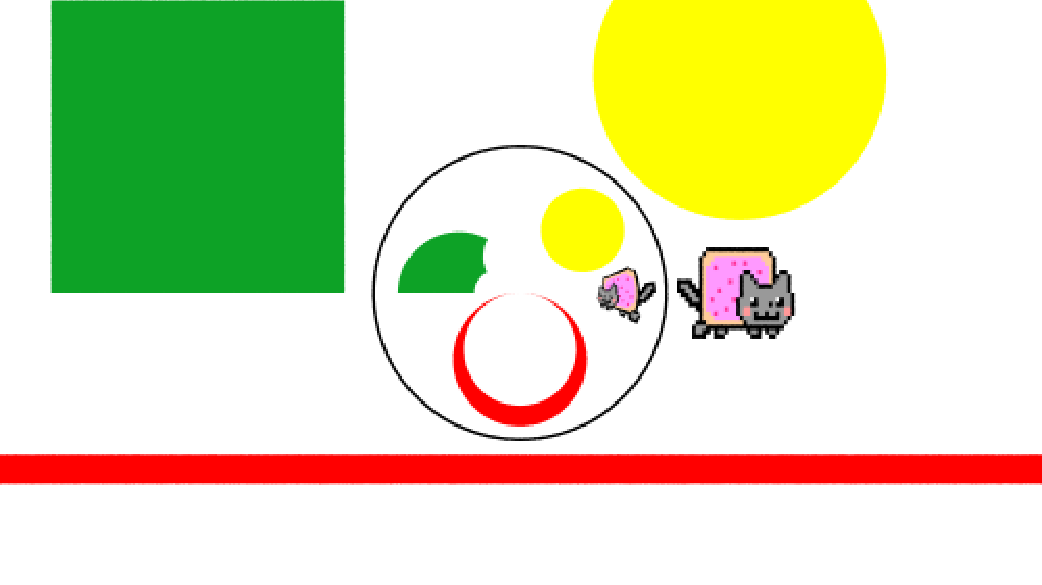
\includegraphics[width=3in, height=3in, keepaspectratio]{../img/klein/circleInversion.pdf}
    \caption{Circle Inversion}
    \label{fig:circleInversion}
 \end{center}
\end{figure}

メビウス変換はおおまかに\emph{放物型}, \emph{斜航型},\emph{楕円型}の三種類に分類される.
斜航型変換と楕円型変換は2つ,放物型変換は1つの固定点をもつ.
斜航型変換は単純な回転を除いた複素数によるスケーリングと共役である.
また斜航型変換の中でも,スケーリングの係数が正の実数であるとき,その変換を\emph{双曲型}と呼ぶ場合もある.
放物型は平行移動と共役で, 楕円型変換は回転と共役である.

クライン群の描画において,メビウス変換の分類は重要である.
なぜならば,楕円型変換を含む群の多くはクライン群にはなりえない.
また,放物型変換は固定点への収束が遅いという特徴をもつ.
これは後述する極限集合の描画の際に考慮することとなる.

メビウス変換は4つの複素数で構成されていることから,8つのパラメータがある.ただし,このままでは自由度が高すぎるため,適切に制限を加えた群の「レシピ」が作られている.
『インドラの真珠』で使われる「おばあちゃんのレシピ」をみてみよう.
\begin{eqnarray*}
 t_a, t_b \in \mathbb{C} \\
 x^2 - t_a t_b x + t_a^2 + t_b^2 = 0 \text{の一方の解}x\text{を}t_{ab} = x \text{とする. }\\
 z_0 = \frac{(t_{ab} -2)t_b}{t_b t_{ab} - 2 t_a + 2it_{ab}}\\
 A = \left(
      \begin{array}{ccc}
       \frac{t_a}{2} & \frac{t_a t_{ab} - 2 t_b + 4i}{(2 t_{ab} + 4)z_0} \\
       \frac{(t_a t_{ab} - 2 t_b -4i)z_0}{2 t_{ab} - 4} & \frac{t_a}{2}
      \end{array}
     \right)
 B = \left(
      \begin{array}{ccc}
       \frac{t_b - 2i}{2} & \frac{t_b}{2} \\
       \frac{t_b}{2} & \frac{t_b + 2i}{2}
      \end{array}
     \right)
\end{eqnarray*}
パラメータは二つの複素数$t_a, t_b$と$t_{ab}$の選び方となった.
「おばあちゃんのレシピ」は群を可視化した際に綺麗な図がレンダリングされるように調整がなされている.

\subsection{Stereographic Projection}

拡張複素平面はリーマン球面という名の通り, 球面で表すことで全
体をよく見ることができる.
地図の制作のため, 地球のような球面を平面に投影する方法が様々に考えられて
きたが, 複素平面を球面へと写像するためには, \emph{立体射影}({\it
stereographic projection})と呼ばれる方法がよく使われる.
立体射影は角度と円を保つため, メビウス変換と相性が良い.
立体射影では, 無限遠点は北極へ, 原点は南極へと移る.
北極から他の球面上の点へと直線を引く.
その直線と平面の交点が立体射影により移り合う点である.
図\ref{fig:stereoProject}は立体射影を図示したものである.
赤の円は単位円を表す. 単位円は赤道へと移る.

Saul Schleimer, Henry Segermanはこれを利用した全天球画像へのエフェクトを
考案している\cite{spherical}.
図\ref{fig:spherical}は正距円筒図法(Equirectangular map)と球の内側からみ
た視点と, 複素平面とリーマン球面を可視化したものである.
このように, 複素平面上での回転は球の回転として表わすことができる.
\footnote{Spherical Droste video: \url{https://www.youtube.com/watch?v=qvh-EAipIUk\&t=4s}}

\begin{figure}[htbp]
 \center
 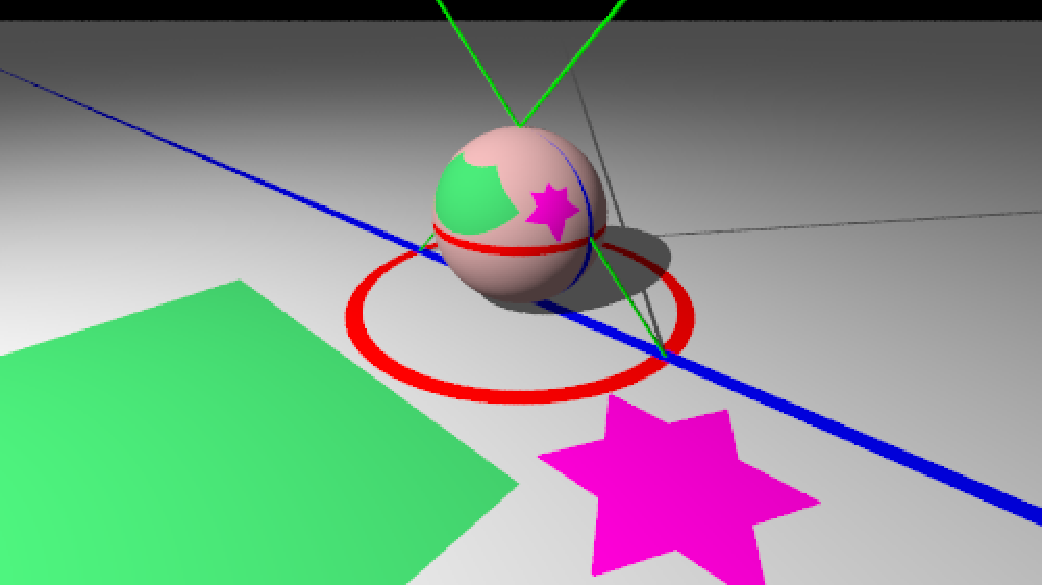
\includegraphics[width=3in, height=3in, keepaspectratio]{../img/klein/stereoProject.pdf}
 \caption{Stereographic Projection}
 \label{fig:stereoProject}
\end{figure}

\begin{figure}[htbp]
 \begin{minipage}{0.5\hsize}
  \center
  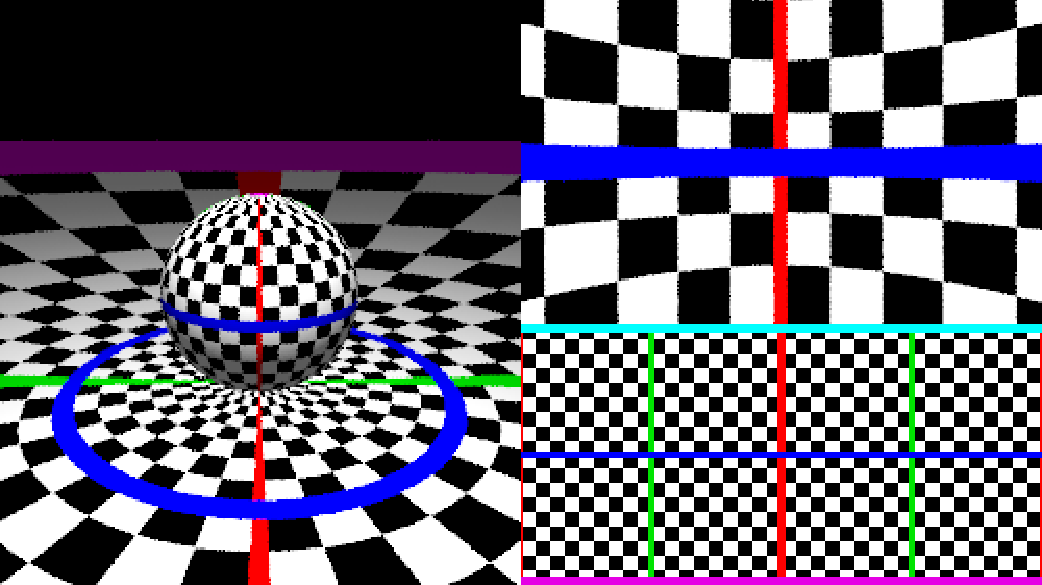
\includegraphics[width=3in, height=3in, keepaspectratio]{../img/klein/spherical.pdf}
  \subcaption{Stereographic }
  \label{fig:sphericalStandard}
 \end{minipage}
 \begin{minipage}{0.5\hsize}
  \center
  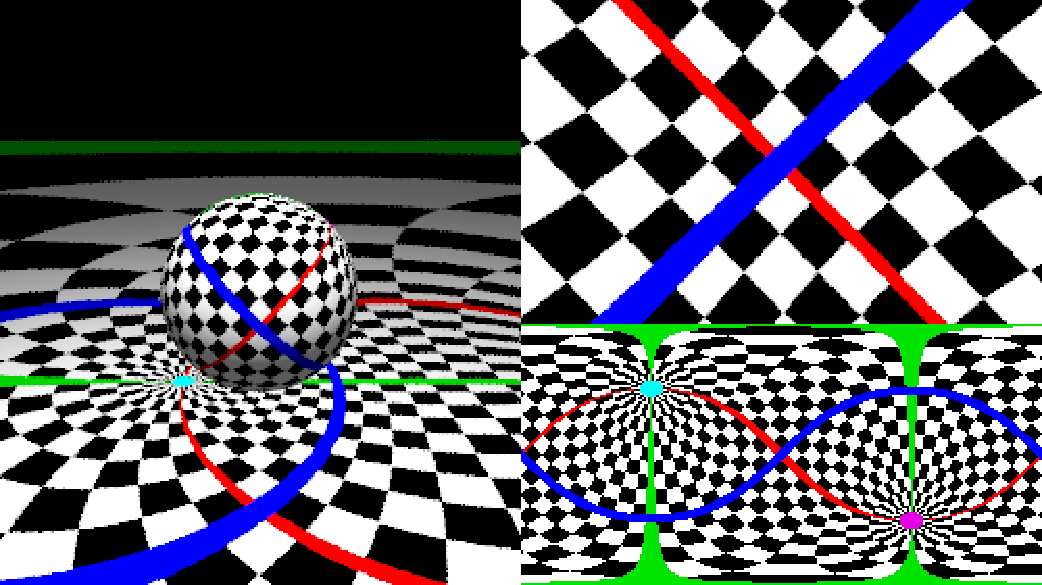
\includegraphics[width=3in, height=3in, keepaspectratio]{../img/klein/sphericalRotation.pdf}
  \subcaption{Stereographic 2}
  \label{fig:sphericalRotation}
 \end{minipage}
 \caption{Spherical image}
 \label{fig:spherical}
\end{figure}

\subsection{Graph Traversal Approach}

群を構成する変換の全組み合わせを調べるとき,変換の語で構成される木構造を考える.
図\ref{fig:wordTree}のような木はケーリーグラフ(Cayley graph)と呼ばれ4種類の変換の合成の組合せを表わしている.
この木を探索することで得られる合成変換を用いて群の作用を可視化する.
ここでは簡単にその方法をまとめる.
疑似コードを含む詳細な解説は『インドラの真珠』にある.

\begin{figure}[htbp]
 \center
 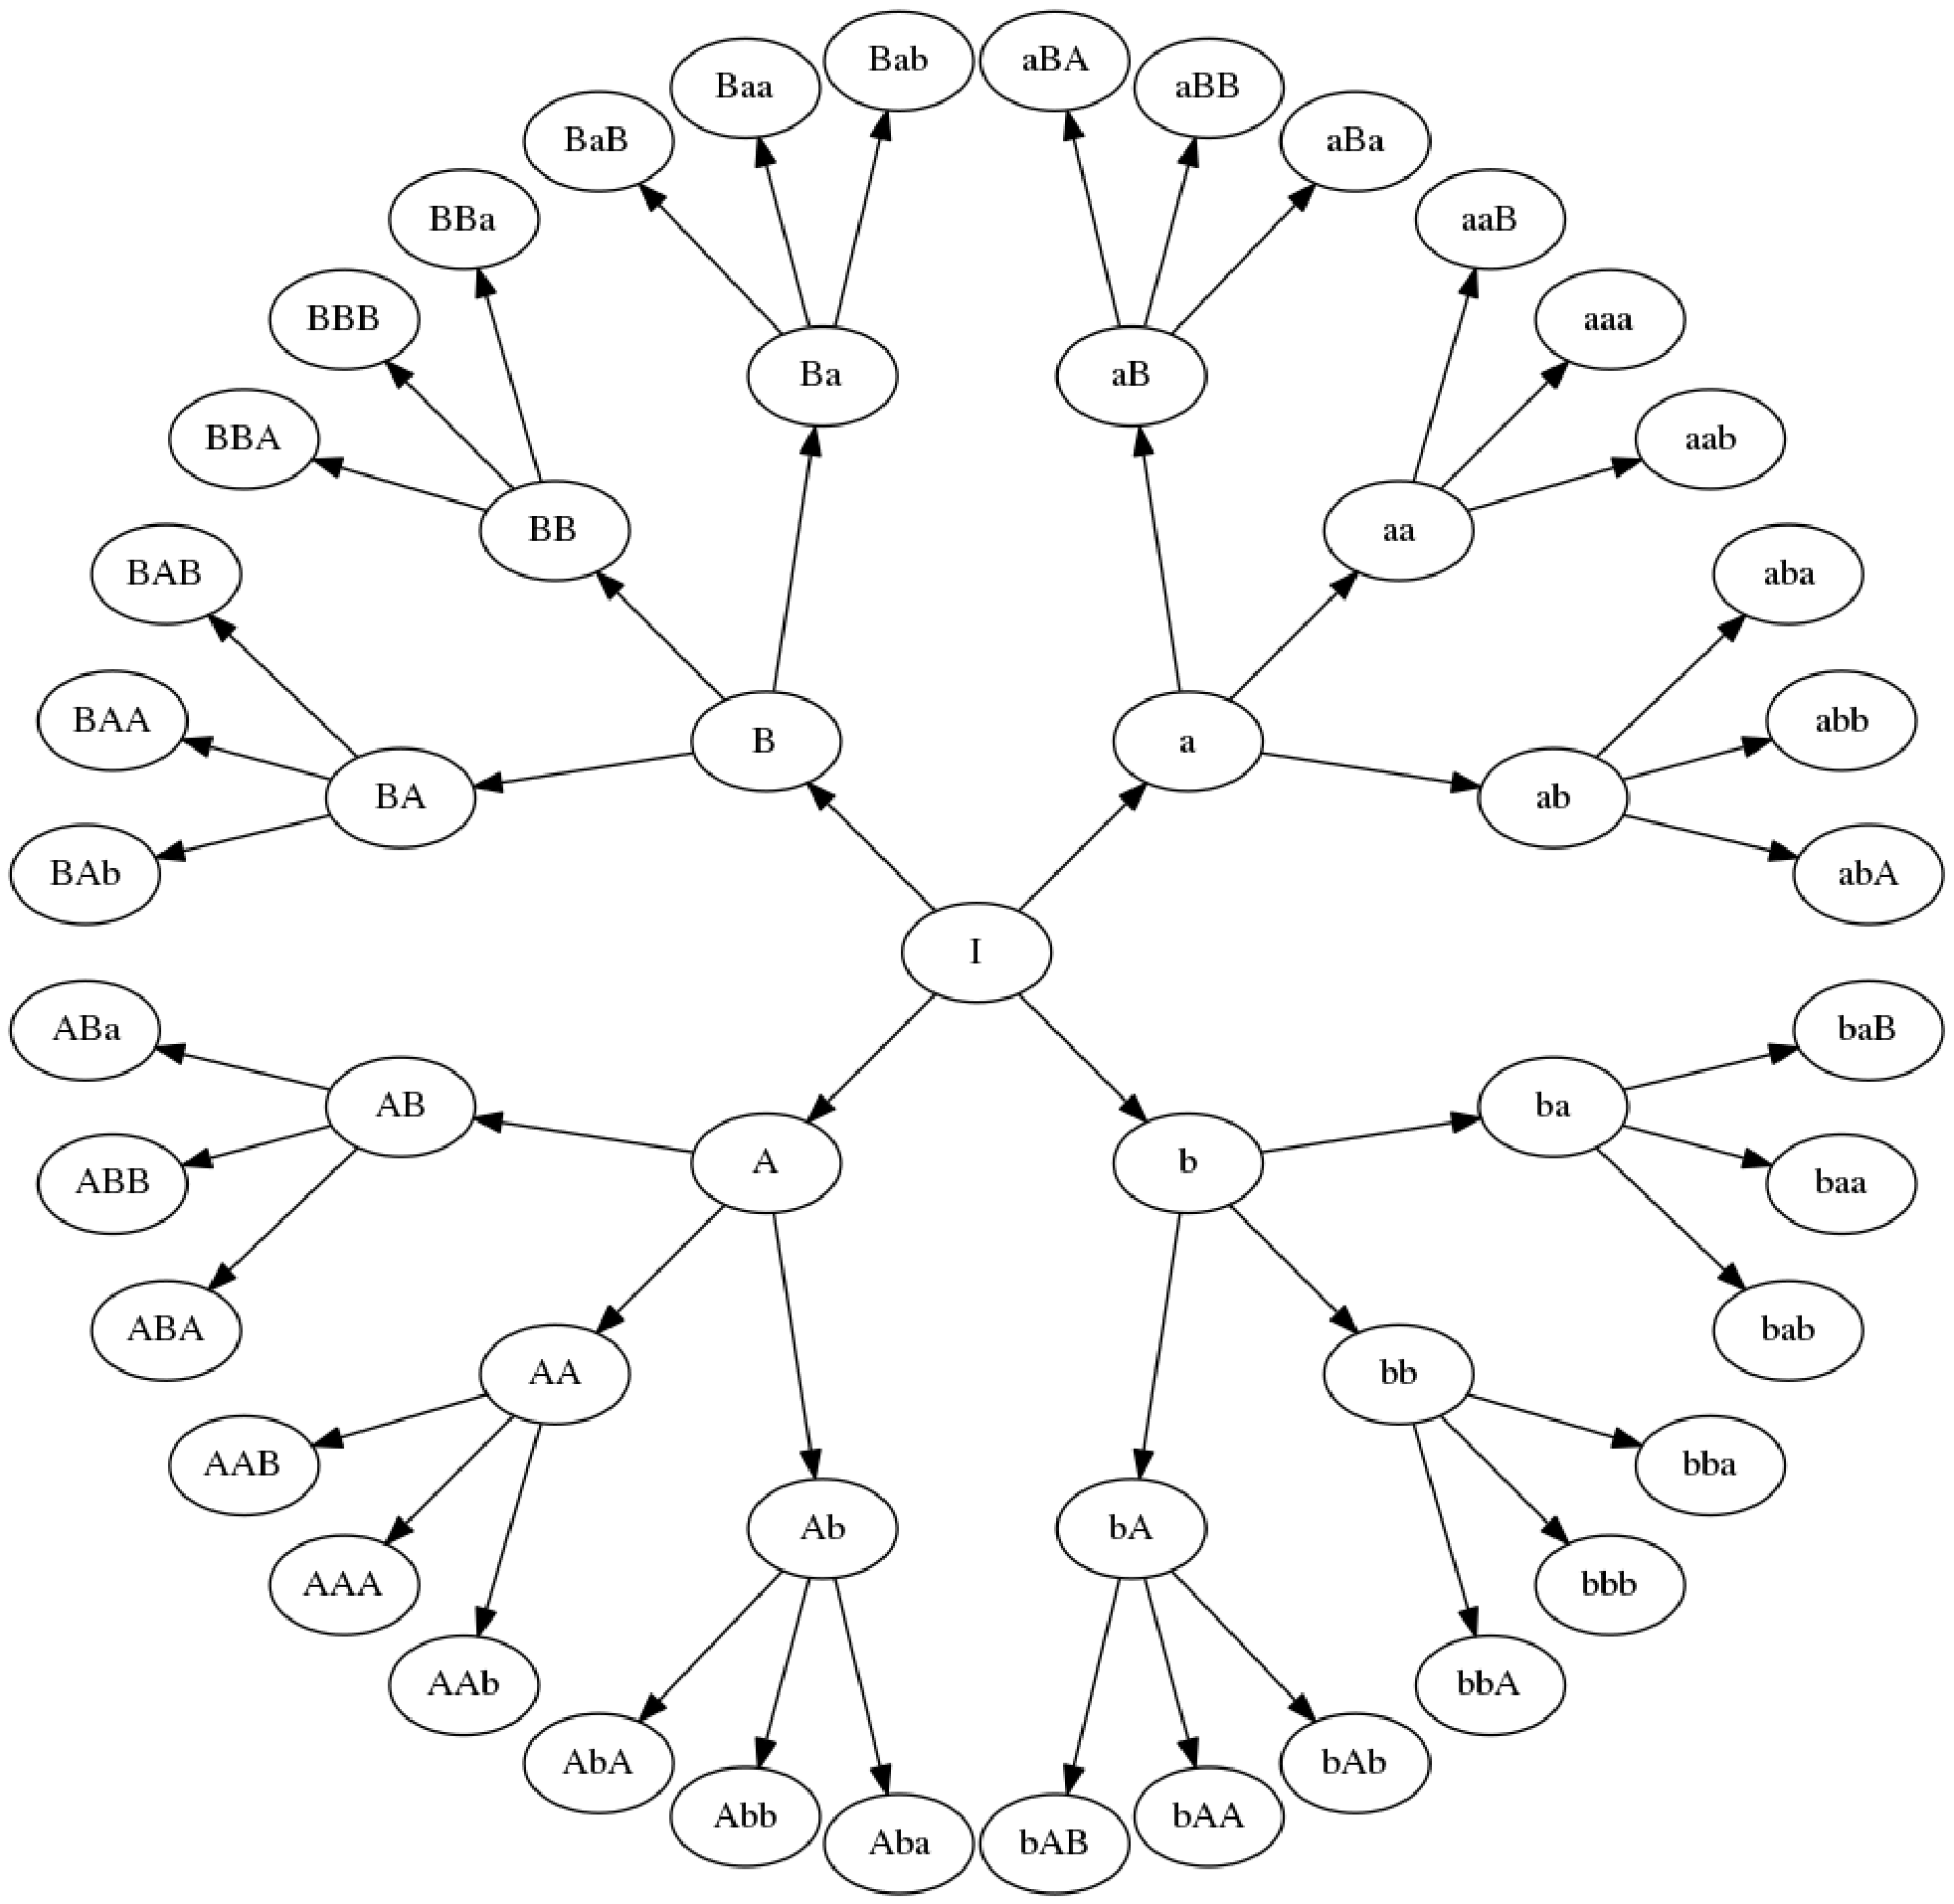
\includegraphics[width=3in, height=3in, keepaspectratio]{../img/klein/wordTree.pdf}
 \caption{Word Tree}
 \label{fig:wordTree}
\end{figure}

\subsubsection{Rendering the Orbit of Transformations}

まず, 円の反転で構成される群を可視化してみよう.
円の反転は変換自体を円という図形で表現できるため, その作用を理解しやすい.
図\ref{fig:schottky}には4つ円の内側にたくさんの円が描かれている.
外側にある4つの大きな円を反転円と呼ぶ.
それぞれの反転円の反転は自分以外の反転円を自分の内側に移す.
よって,それぞれの反転円の内側には3つの円が移され,合せて12個の小円ができる.
新たにできた小円に対してもその小円が属している反転円以外の反転を適用することで, 小円の下に新たな小円ができる.
このことを繰り返すと,図\ref{fig:schottky}のように,円が入れ子状につらな
る図を得ることができる.
これが群の生成元による軌道である.
また,円列の極限を極限集合とよぶ.
この極限を観察することがクライン群を研究する上で役に立つ.

図\ref{fig:schottky}では反転円の軌道を描いが, 同様にして違う図形の軌道を描くこともできる.
例えば, 図\ref{fig:orbit}は中央に置いた猫の画像を4つ反転円による反転で移した軌道を描いた.
図\ref{fig:apr}はP.Nylander氏による作品\footnote{bugman123.com Fractals: \url{http://bugman123.com/Fractals/index.html}}を参考に描画した.
中央右側の蝶をおばあちゃんのレシピで得られた群の生成元で移した.
虹色の曲線は極限集合である.
どちらの図も図形の軌道は最終的に極限集合へと収束していくことがわかる.

このアルゴリズムは変換で構成される木構造を幅優先探索で探索することに等しい.
例えば, 図\ref{fig:wordTree}の語の木を時計回りに探索すると$a, b, A, B, aB, aa, ab, ba, bb, ...$の順に合成された変換を得ることができる.
あらかじめ決められた深さまで調べたら, 得られたすべての変換の語を大本となる図形(図\ref{fig:orbit}における中央の猫)に対して適用することで, おおまかに生成元の作用を調べることができる.


\begin{figure}[htbp]
 \begin{minipage}{0.49\hsize}
  \begin{center}
   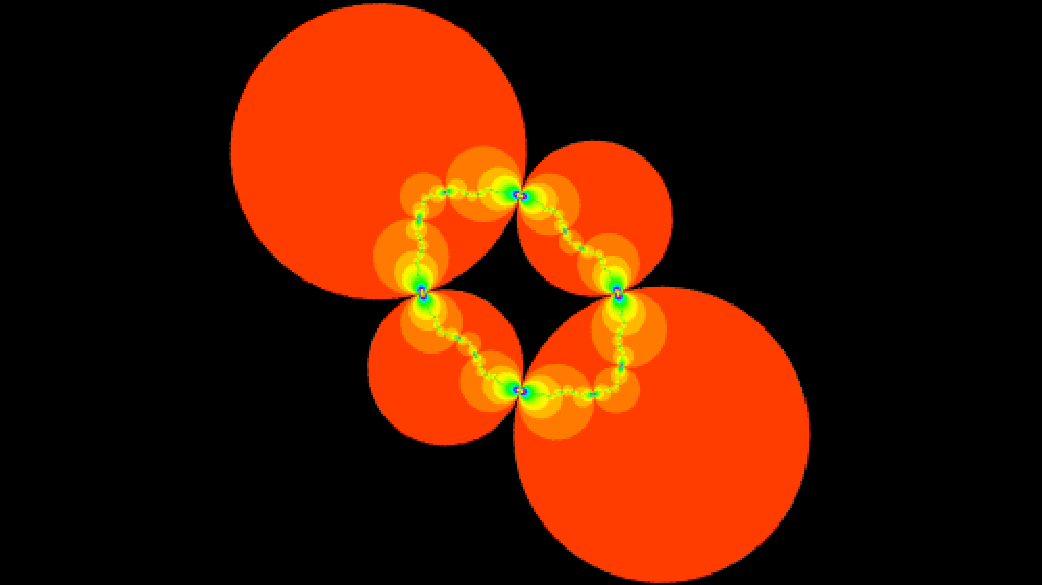
\includegraphics[width=3in, height=3in, keepaspectratio]{../img/klein/schottkyCircles.pdf}
   \caption{Schottky Circles}
   \label{fig:schottky}
  \end{center}
 \end{minipage}
 \begin{minipage}{0.49\hsize}
  \begin{center}
   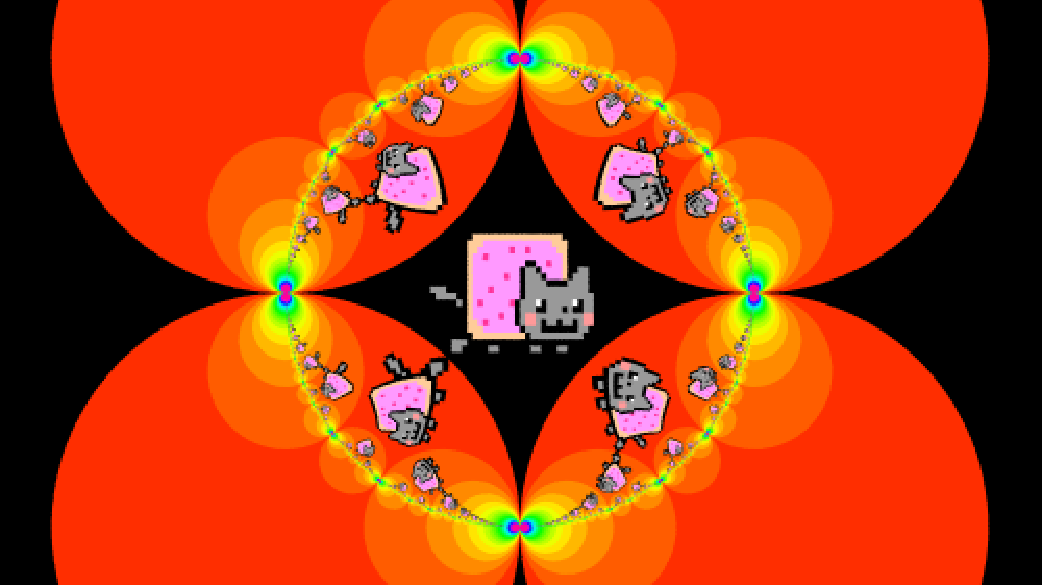
\includegraphics[width=3in, height=3in, keepaspectratio]{../img/klein/circleOrbit.pdf}
   \caption{orbit}
   \label{fig:orbit}
  \end{center}
 \end{minipage}
\end{figure}


\subsubsection{Rendering the Limit Set}

前節でみた極限集合を直接描くこともできる.
全てのメビウス変換に円の反転における円のような図形を考えることは難しいので, 研究では主にこの方法が使われている.
極限集合は群の生成元の固定点をある程度の長さをもった変換の語で移すことで求めることができる.
例えば, 変換$a$の固定点は任意の点に$a$を繰り返し適用した点, つまり$\overline{a}$を適用した極限点と考えることができる.
よって, 変換$abbAAb\overline{a}$で表わされる極限点は$a$の固定点を合成変換$abbAAb$で移すことで求めることができる.
この時, $abbAAb$を接頭語と呼ぶ.

図\ref{fig:wordTree}の語の木を時計回りに長さ3までの語を探索すると,$ aBA, aBB, aBa, aaB, ...$という順で接頭語が得られる.
これらの語に, 逆変換をかけないように, 生成元の固定点を与えると極限点を求めることができる.
例えば$aBA$を用いて$\overline{A}, \overline{b}, \overline{B}$の3つの固定点を変換すると互いに近い3つの極限点が得られる.
$aab\overline{a}$と$aaa\overline{a}$のように隣同士の接頭語を持つ極限点や $aaa\overline{a}$と$aaa\overline{b}$のような同じ接頭語を持つ極限点同士は近い.
そのため, 得られた点同士を順番に結ぶと図のようなフラクタル構造を持つ曲線を得ることができる.
実際に実装する場合には, 得られた点同士の距離によってより深い語への探索の打ち切りと継続を決める.

ただし, 綺麗に描画するには様々な工夫が必要となる.
まず, 放物型変換は固定点への収束に時間がかかため, 放物型変換の固定点付近をうまく描画するためには, 放物型の生成元のための特別な処理が必要である.
図\ref{fig:apr}の右端をよく見ると直線で結ばれていることがわかる.
ここには放物型変換の固定点が存在しており, 収束が遅いため, この近辺の極限点を得るためには, より長い接頭語が必要となっている.
インドラの真珠では特殊語アルゴリズムと呼ばれるアルゴリズムでこの問題に対処する.

また, ある変換に対してその逆変換をかけてしまうと元にもどってしまうことは自明であるが, 特定の変換の組み合わせが逆戻りを生み出してしまうことがある.
例えば, 先に述べた平行移動の例において,abABという変換は点を一周させて元の場所に戻してしまう.
このような変換をもたない群を\emph{自由群}と呼ぶ.
効率よく描画するためには,うまくこのような元を取り除く必要がある.これを解決するためには有限オートマトンが使われる.
インドラの真珠においても有限オートマトンの使い方に関する解説はあるが, より数学的な事項は『Word Processing In Groups』\cite{wordProcessing}が詳しい.

先に述べたように,メビウス変換の群すべてがクライン群になるわけではない.
群のレシピのパラメータの中には描画すると極限集合が収束せず,図
\ref{fig:non-discrete}のように乱れるようなものがある.
このような群は非離散群と呼ばれ,クライン群ではない.
この離散と非離散のパラメータ領域を描画した図は'スライス'と呼ばれる.
スライスの離散と非離散の境界もフラクタル形状となる.
境界のパラメータを用いて描画するとしばしば極限集合が興味深い形になる.
山下靖氏のページ\footnote{Discreteness Locus:
\url{http://vivaldi.ics.nara-wu.ac.jp/~yamasita/Slice/}}では様々なスライ
スを見ることができる.
どのようなパラメータが離散的であるか,すなわちクライン群となるかを調べることがクライン群の研究テーマの一つとなる.


\begin{figure}[h!tbp]
 \begin{subfigure}{0.49\hsize}
   \begin{center}
    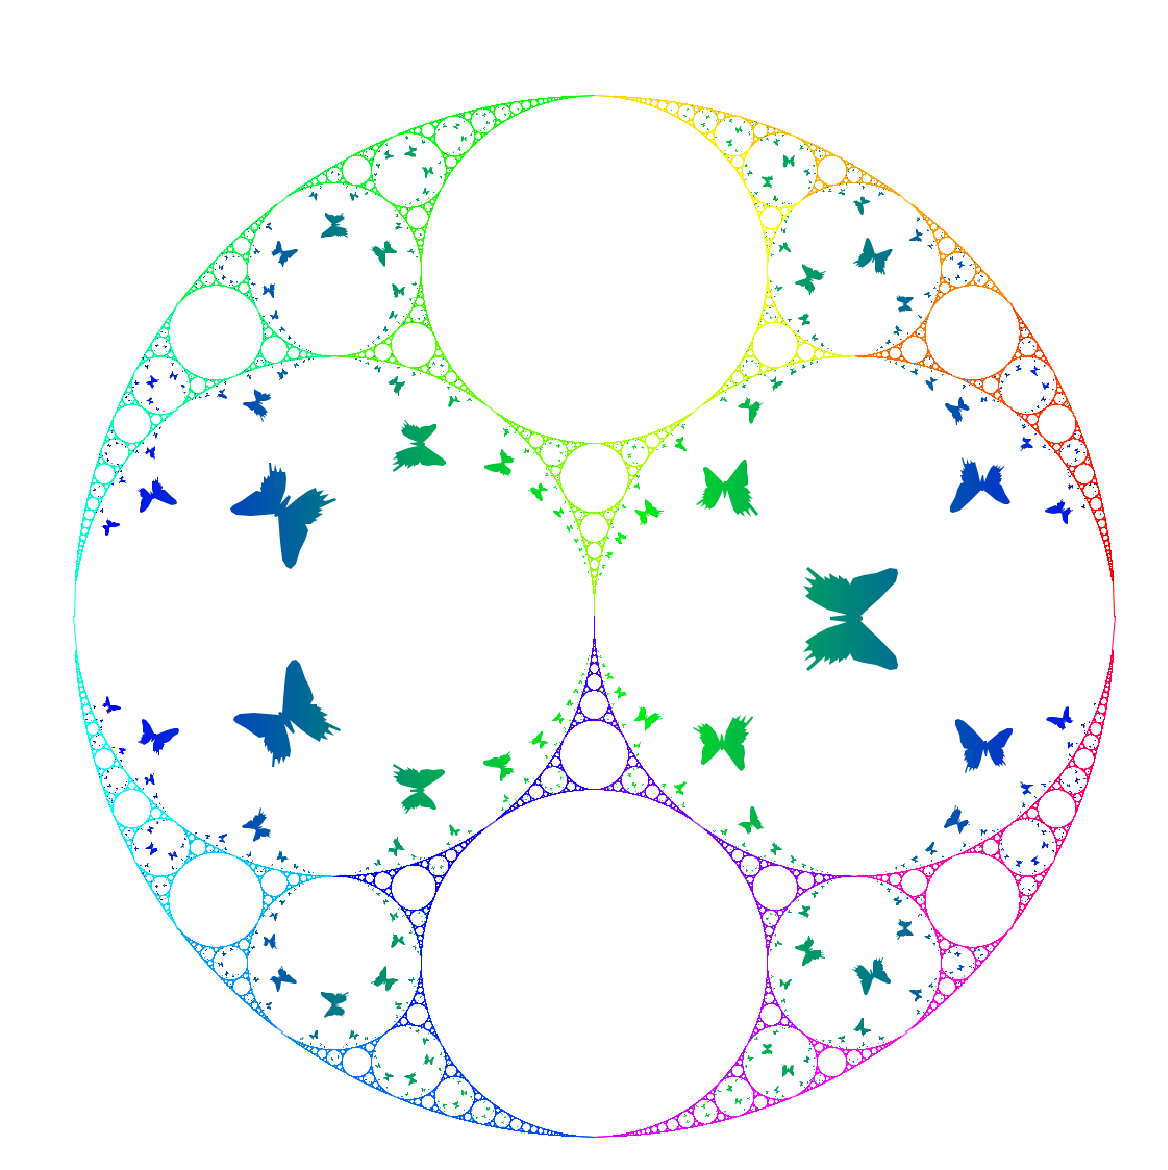
\includegraphics[width=3in, height=3in, keepaspectratio]{../img/klein/apr.pdf}
    \caption{}
    \label{fig:apr}
   \end{center}
 \end{subfigure}
 \hspace*{\fill}
 \begin{subfigure}{0.49\hsize}
   \begin{center}
    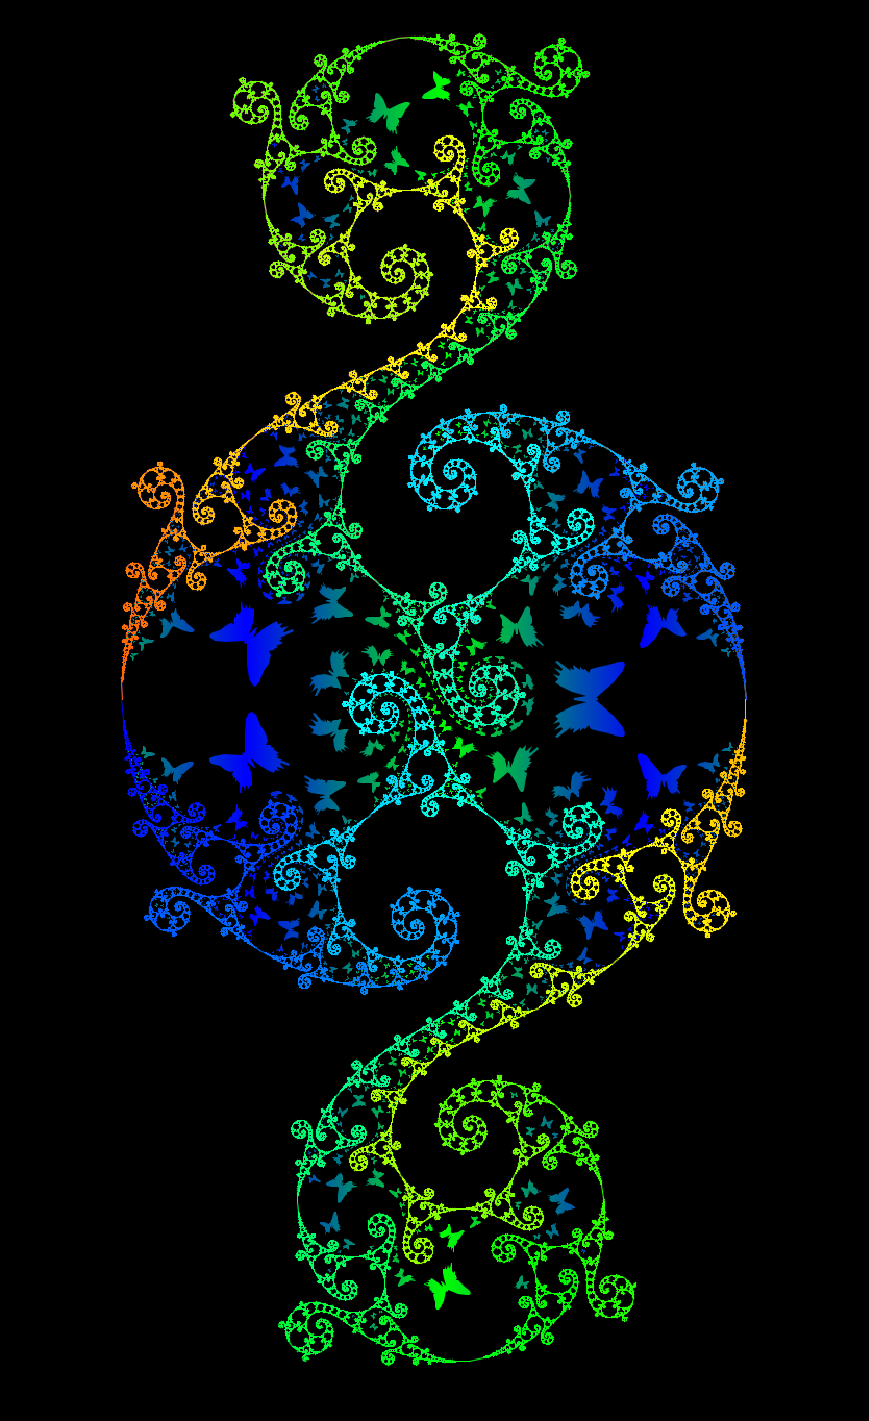
\includegraphics[width=3in, height=3in, keepaspectratio]{../img/klein/comp.pdf}
    \caption{}
    \label{fig:comp}
   \end{center}
 \end{subfigure}
 \caption{The limit set of Kleinian Groups}
 \label{fig:limitsetWithOrbit}
\end{figure}

\begin{figure}[htbp]
 \begin{subfigure}{0.49\hsize}
  \begin{center}
   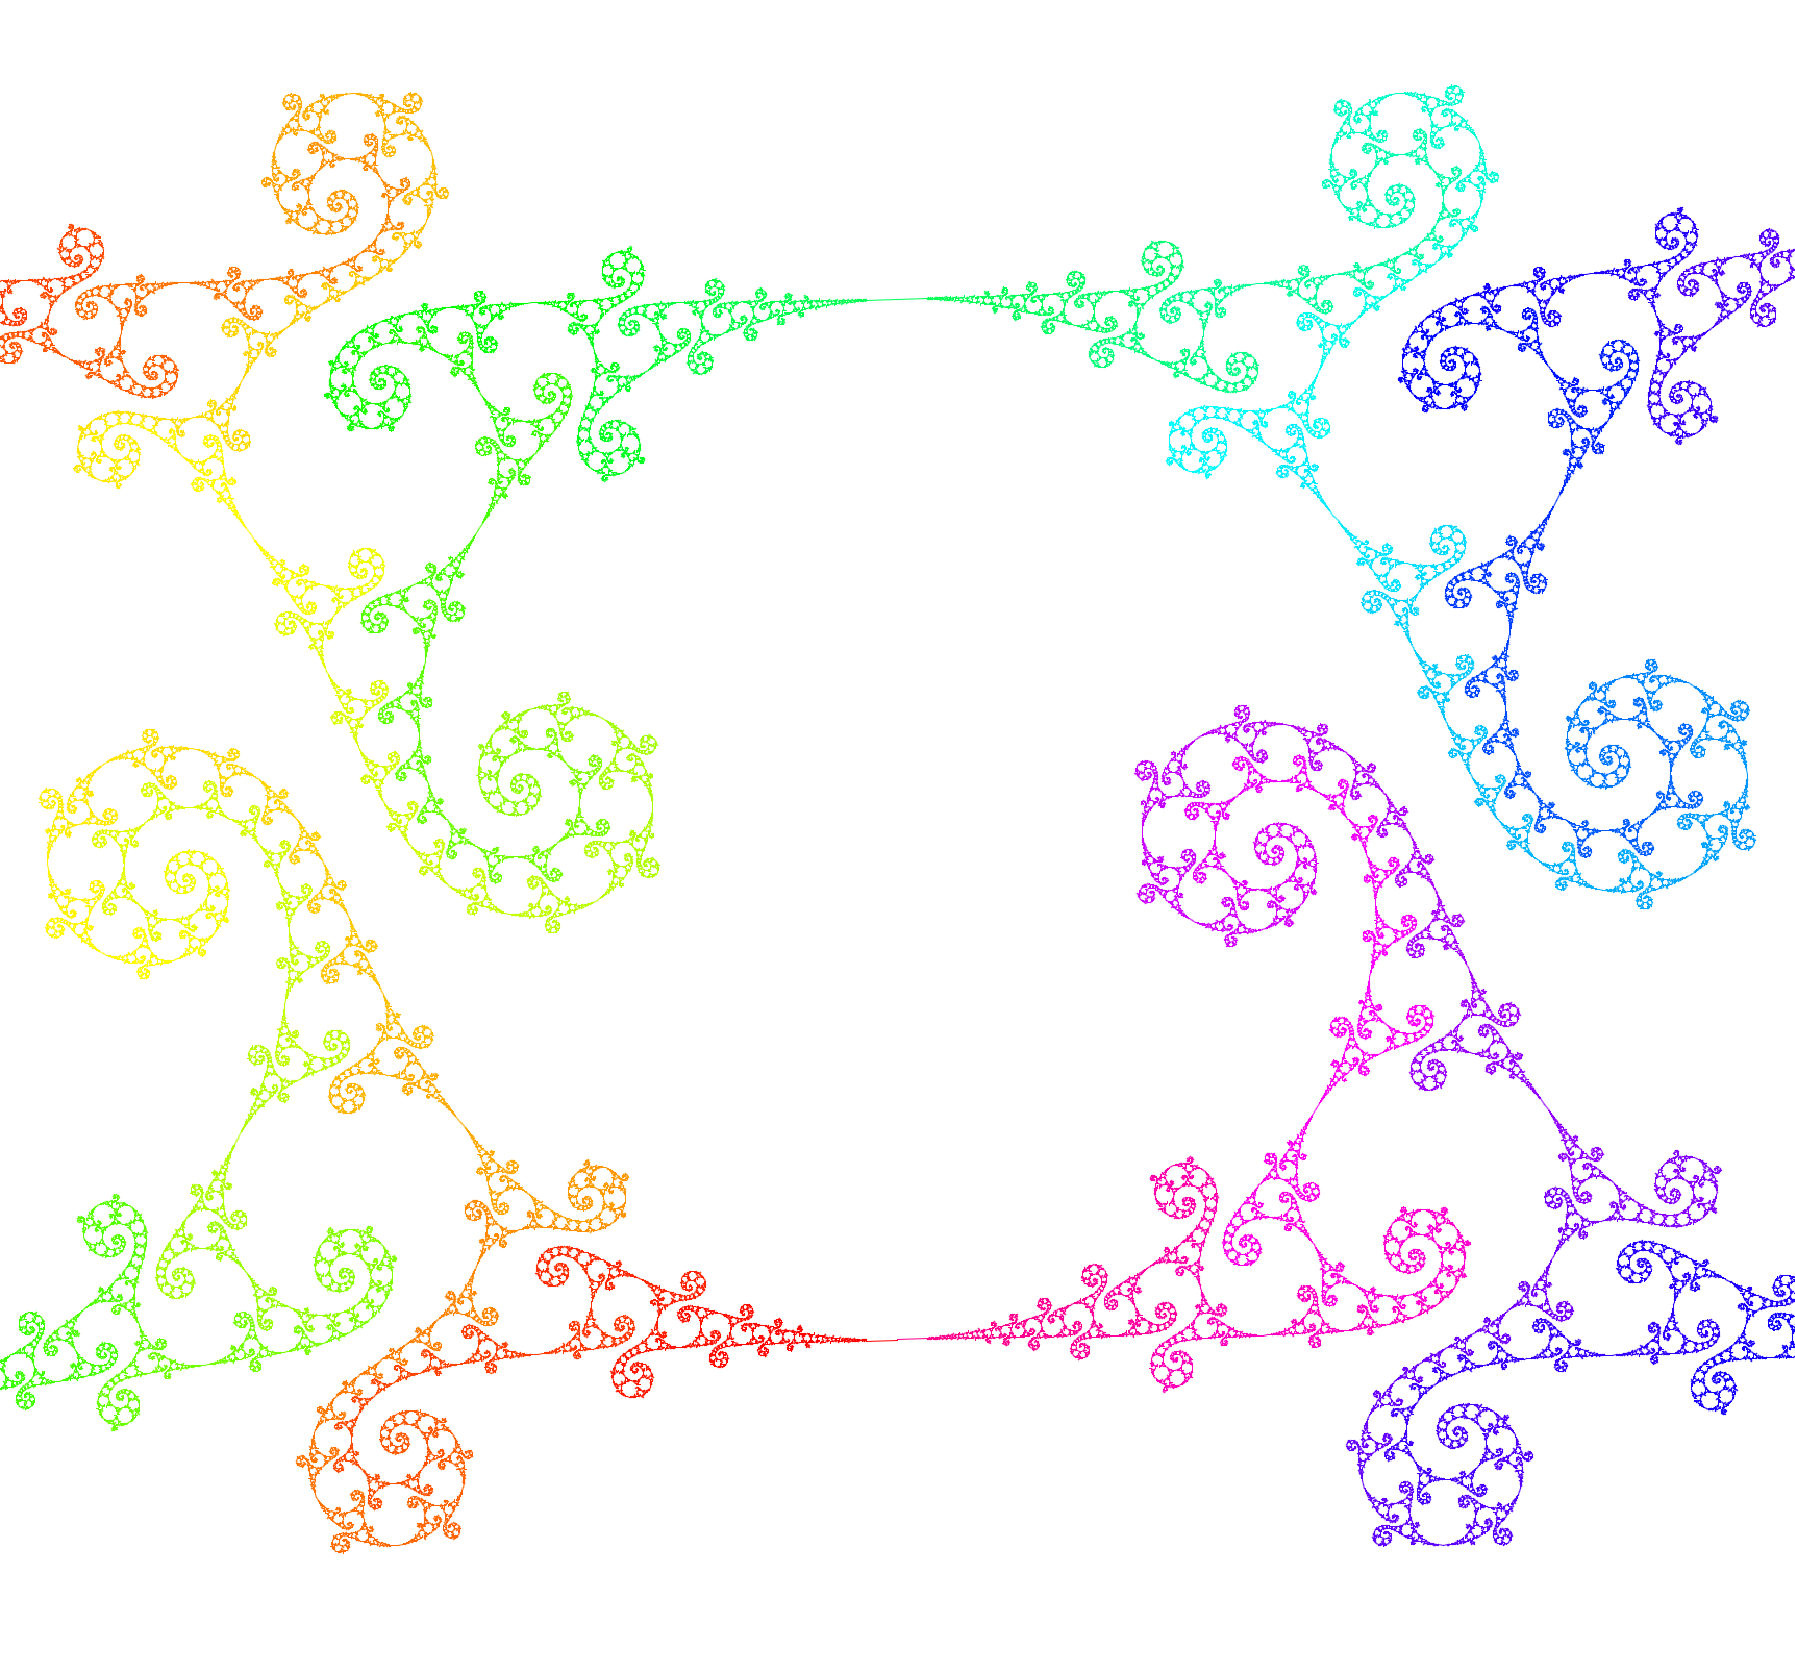
\includegraphics[width=3in, height=3in, keepaspectratio]{../img/klein/horizon.pdf}
   \caption{}
   \label{fig:horizon1}
  \end{center}
 \end{subfigure}
 \begin{subfigure}{0.49\hsize}
  \begin{center}
   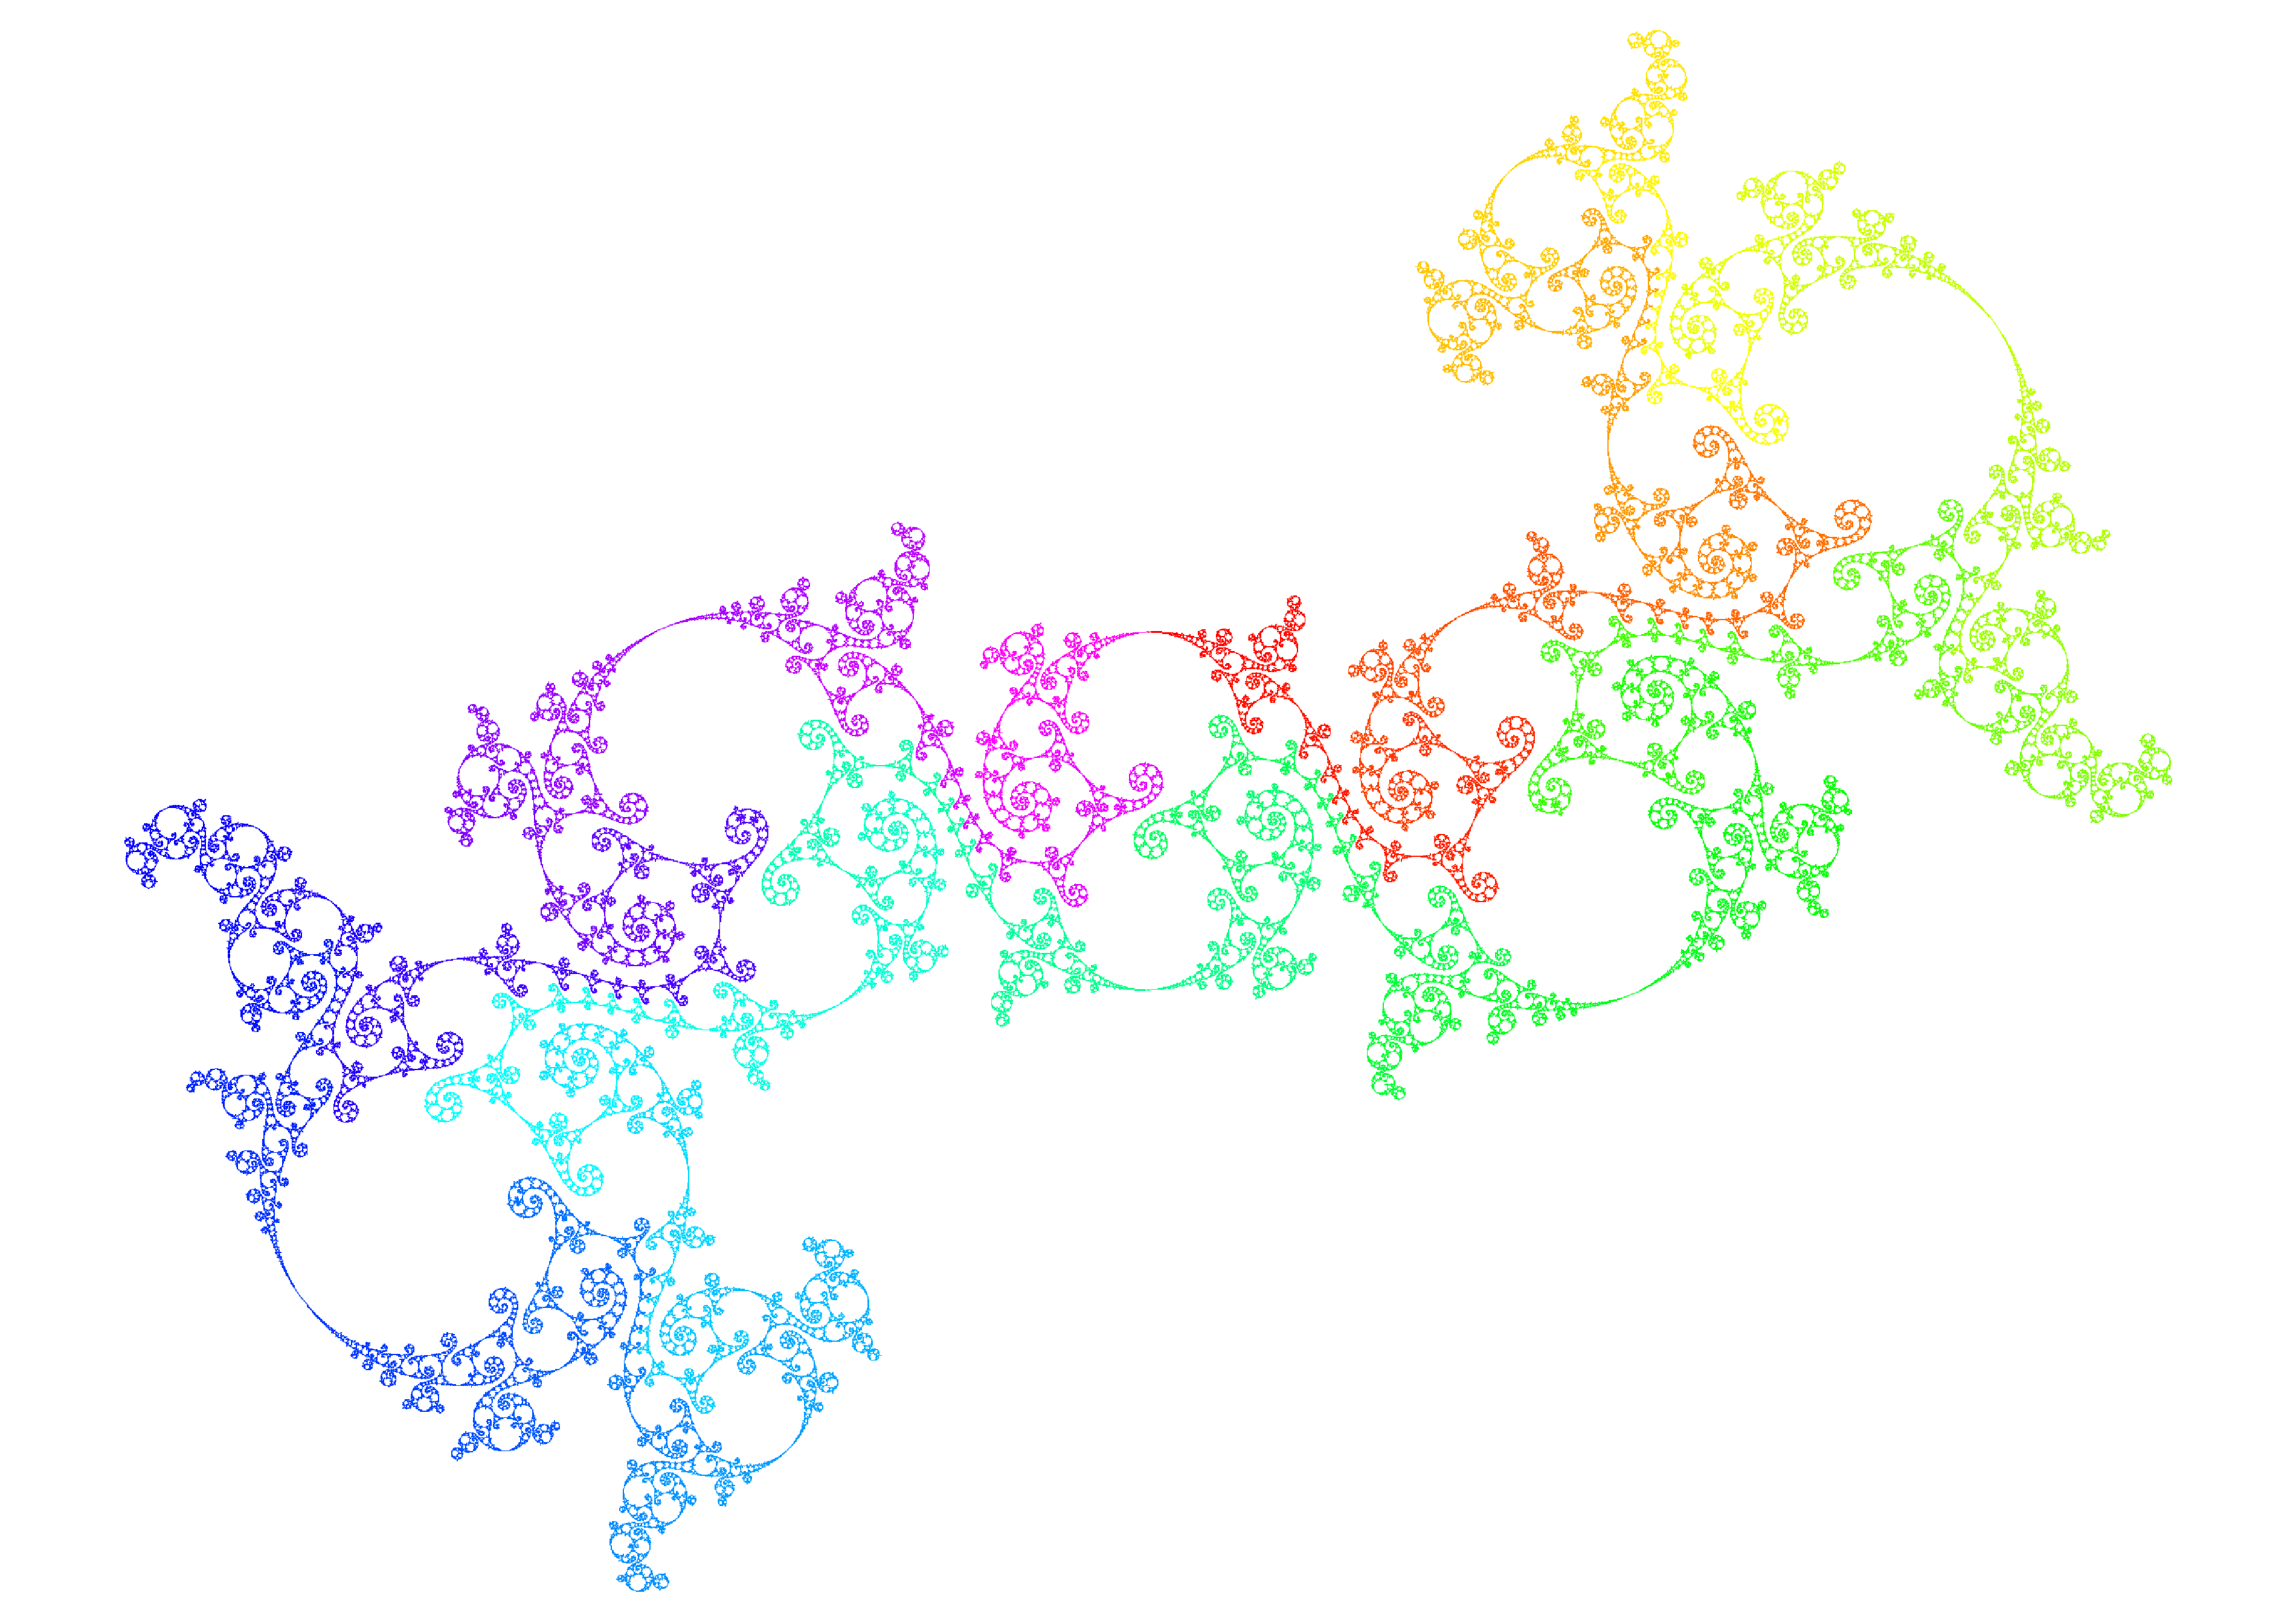
\includegraphics[width=3in, height=3in, keepaspectratio]{../img/klein/limit-horizontal.pdf}
   \caption{}
   \label{fig:horizon2}
  \end{center}
 \end{subfigure}\\
 \begin{subfigure}{0.49\hsize}
  \begin{center}
   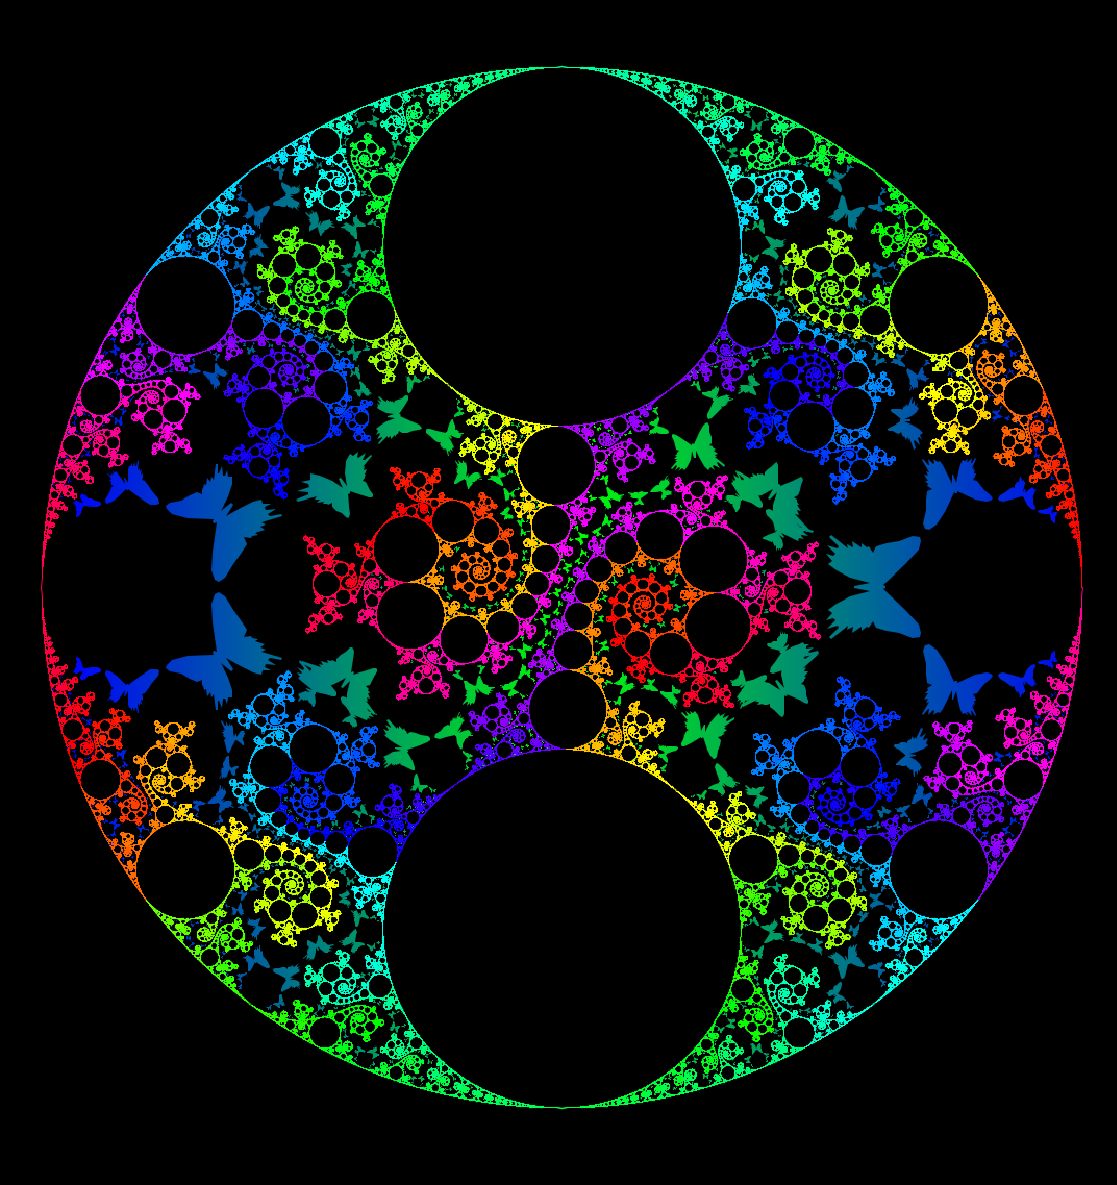
\includegraphics[width=3in, height=3in, keepaspectratio]{../img/klein/limit3.pdf}
   \caption{}
   \label{fig:limit3}
  \end{center}
 \end{subfigure}
 \begin{subfigure}{0.49\hsize}
  \begin{center}
   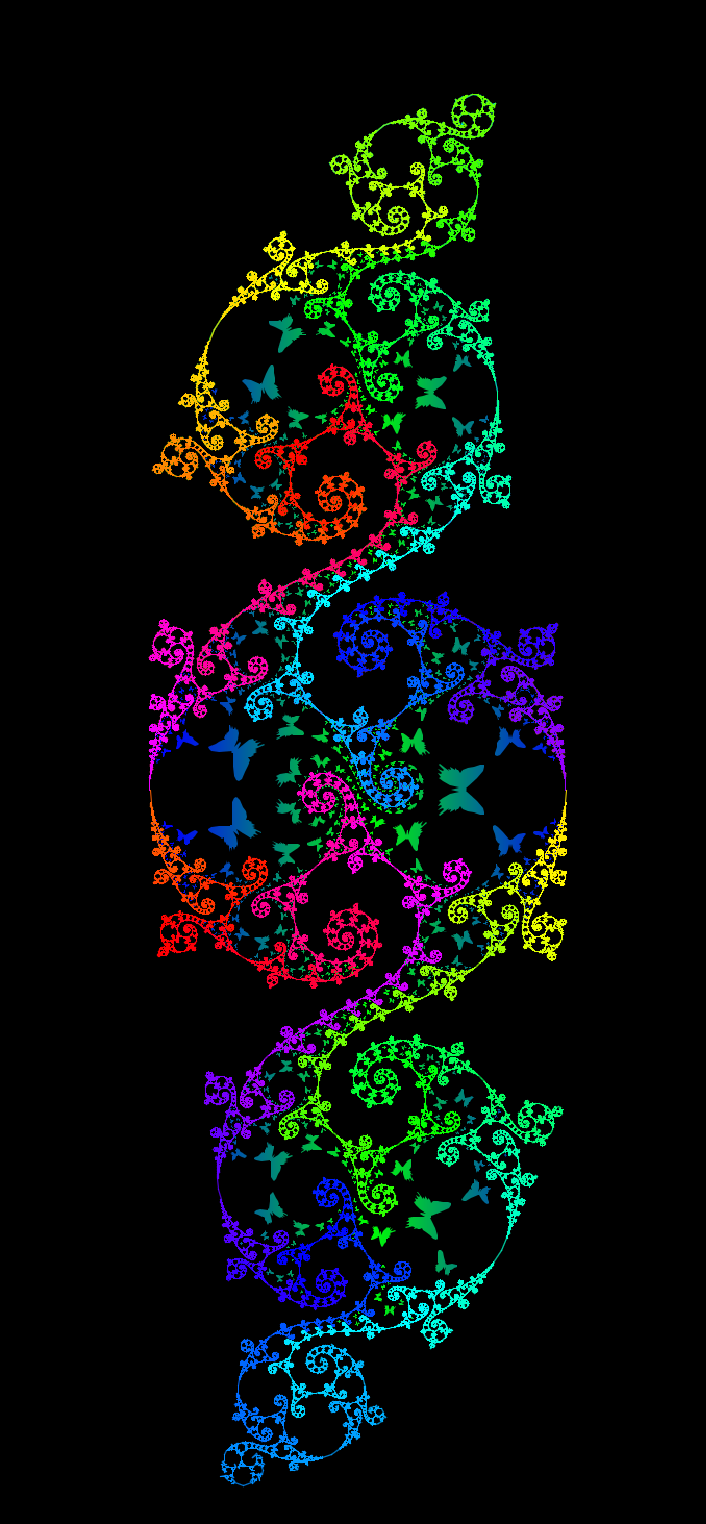
\includegraphics[width=3in, height=3in, keepaspectratio]{../img/klein/limit4.pdf}
   \caption{}
   \label{fig:limit4}
  \end{center}
 \end{subfigure}
 \caption{The limit set of Kleinian Groups}
 \label{fig:limitset}
\end{figure}

\begin{figure}[htbp]
 \begin{center}
  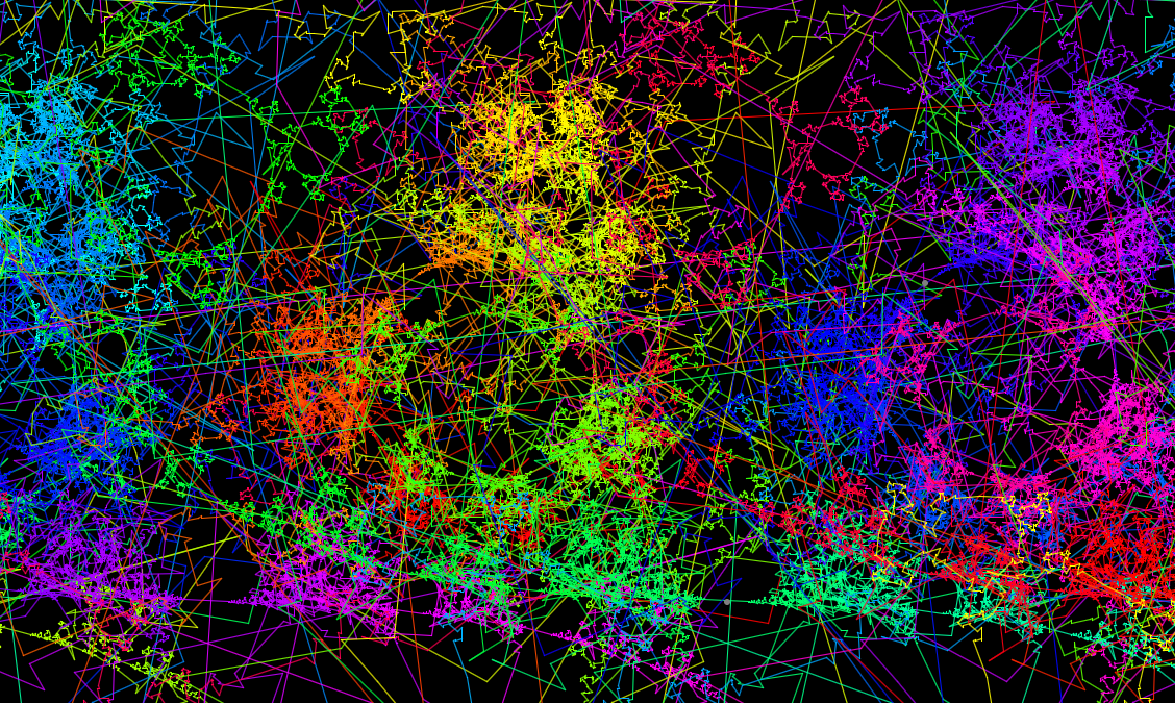
\includegraphics[ height=1.5in, keepaspectratio]{../img/klein/non-discrete.pdf}
  \caption{non discrete}
  \label{fig:non-discrete}
 \end{center}
\end{figure}

\subsubsection{Faults of Graph Traversal Approach}

グラフを探索する方法にはいくつかの欠点がある.
まず, 生成元や,探索を深くするごとに指数オーダーで計算量が増えてしまう.
また, 部分的に拡大したい場合に無駄な部分を計算しないといった処理にも手間
がかかる.
さらに木構造の探索は並列化に向かないため, 高速化が難しい.
そのため, 木構造の探索に頼らない方法がいくつか考案されている.

しかしながら, 最近のOpenCLやCUDAといった並列計算プラットフォームでは
Dynamic Parallelismという機能を用いることで,木構造探索の並列計算を行う
ことが可能である.
ただし, 最新のハードウェアに依存した機能のため, どの計算機環境でも使えるわけではない.

\subsection{Iterated Inversion System}

筆者らは, 1章でみたシェーダを用いたフラクタルのレンダリングアルゴリズム
に着想を得て, 円や球の反転で構成される群の軌道を高速に描画するためのアル
ゴリズム, \textit{Iterated Inversion System (IIS)}\cite{iis}を開発した.
円や球の座標と半径を直接計算するこれまでのアプローチに対して,このアルゴ
リズムは任意の点が属する円や球の深さを特定する.
これはスクリーンスペースのピクセルそれぞれに対して独立に計算することがで
きるのでGLSLによる並列計算,描画を行うことができる.

図\ref{fig:iis-orb}のような4つの反転円を考える.
黒い領域は基本領域とよぶ.
ある点がいずれかの円盤に属している時にその円に関する反転を行なう.
これを反転後の点がすべての円の外側に移されるまで繰り返す.
最終的に, 行なった反転の回数が, その点が属している円盤の深さとなる.
図\ref{fig:iis-orb}では青い点の軌道を描いている.
この点は二回反転が行なわれているので, 反転円から二番目の円に属している.
それぞれの計算はピクセルごとに行なうことができるため, 多項式時間で描画す
ることができる.
実際にこのアルゴリズムを用いてすべての点を基本領域へと移動させるためには,
無限回の反転が必要である. そのため, あらかじめ最大の反転回数を決めておく.
擬似コードをアルゴリズム\ref{iis2d}に示す.

 \begin{algorithm}
  \caption{Iterated Inversion System (IIS)}
  \label{iis2d}
  \begin{algorithmic}
   \REQUIRE count $= 0$ and coordinates $=$ position determined by
   pixel
   \FOR{$i=0$ to MAX\_INVERSION}
   \STATE inFundamentalDomain $\leftarrow$ \TRUE
   \FOR{ each map $G$ in Maps }
   \IF{$G$ is available to coordinates}
   \STATE coordinates $\leftarrow$ $G(\text{coordinates})$
   \STATE INCREMENT count
   \STATE inFundamentalDomain $\leftarrow$ \FALSE
   \ENDIF
   \ENDFOR
   \IF {inFundamentalDomain}
   \STATE BREAK for
   \ENDIF
   \ENDFOR
   \STATE RETURN count
  \end{algorithmic}
 \end{algorithm}

\begin{figure}[htbp]
 \center
 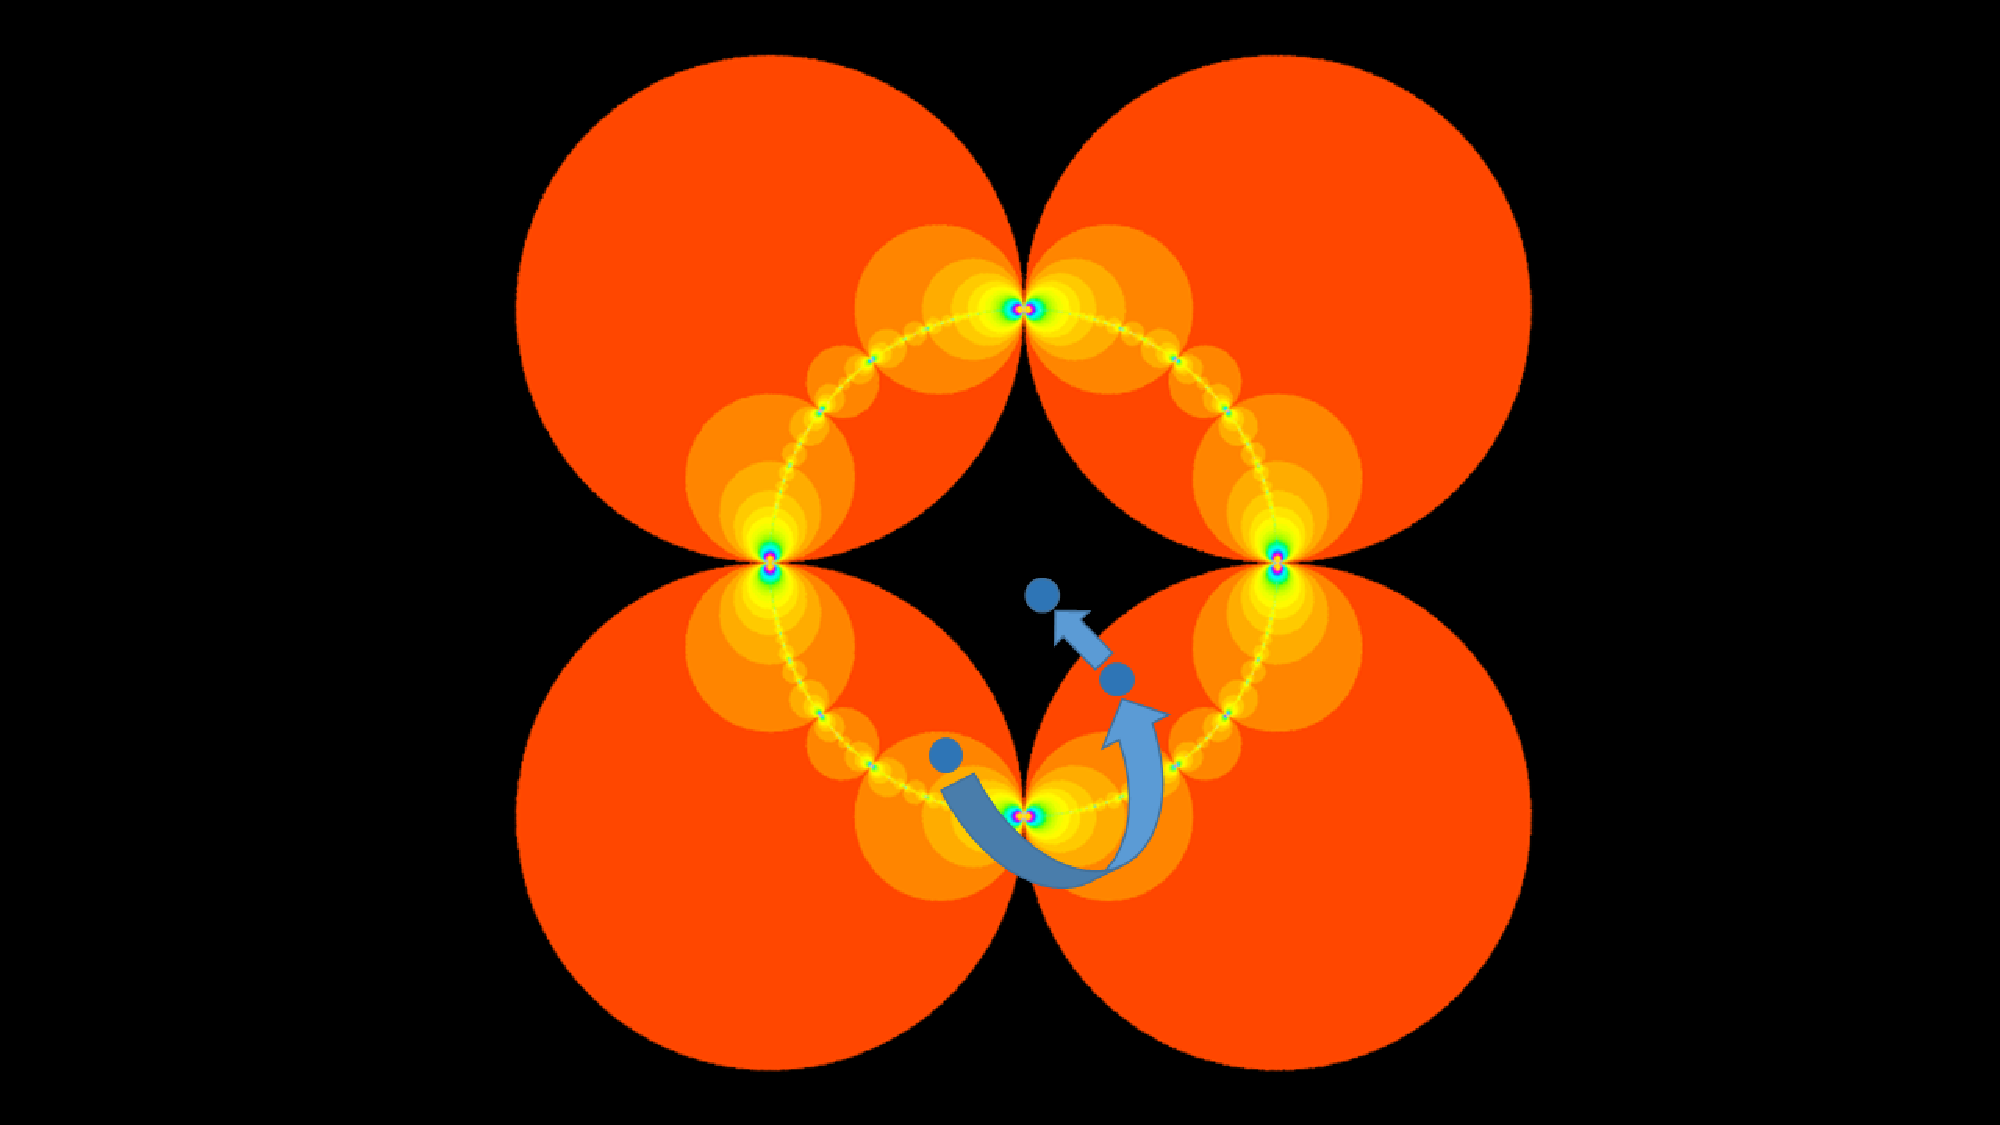
\includegraphics[ height=1.5in, keepaspectratio]{../img/klein/orb.pdf}
 \caption{Orbit}
 \label{fig:iis-orb}
\end{figure}

また, 球の反転による三次元形状もレイマーチングを用いることで, 高速に描画
することができる.
二次元の場合と同様に球の反転によるショットキー球の軌道を描こうとすると,
軌道はショットキー球の内側に連なってしまい, 描画に手間がかかる.
そこで我々は軌道の元となる球を用意し, その球をショットキー球の反転で移し
た軌道を描画する.
図\ref{fig:simpleGen3d}における灰色の球を\emph{ショットキー球},緑色の球を\emph{基本球}とよぶ.
基球をすべてのショットキー球の反転で移すと図\ref{fig:simpleOrb3d}のよう
な軌道が得られる.
レイマーチングに用いる距離関数を求めるため,
ここで簡単のために, 図\ref{fig:xySlice}に示されるような図
\ref{fig:iis-orb}のXY平面での断面を考えることにする.
橙色の円列はショットキー球の軌道, 水色の円が基本球の軌道である.
緑色の点$P2$はレイの先端, であるとすると最も近い球は$S2$となる.
しかし, 我々は$S2$の位置と半径は分からない.
基本球である$S1$の位置と半径のみを知っている.

擬似コードはアルゴリズム\ref{iis3d}に示した.


\begin{figure}[htbp]
 \begin{minipage}[b]{0.5\hsize}
  \begin{minipage}[]{0.49\hsize}
   \center
   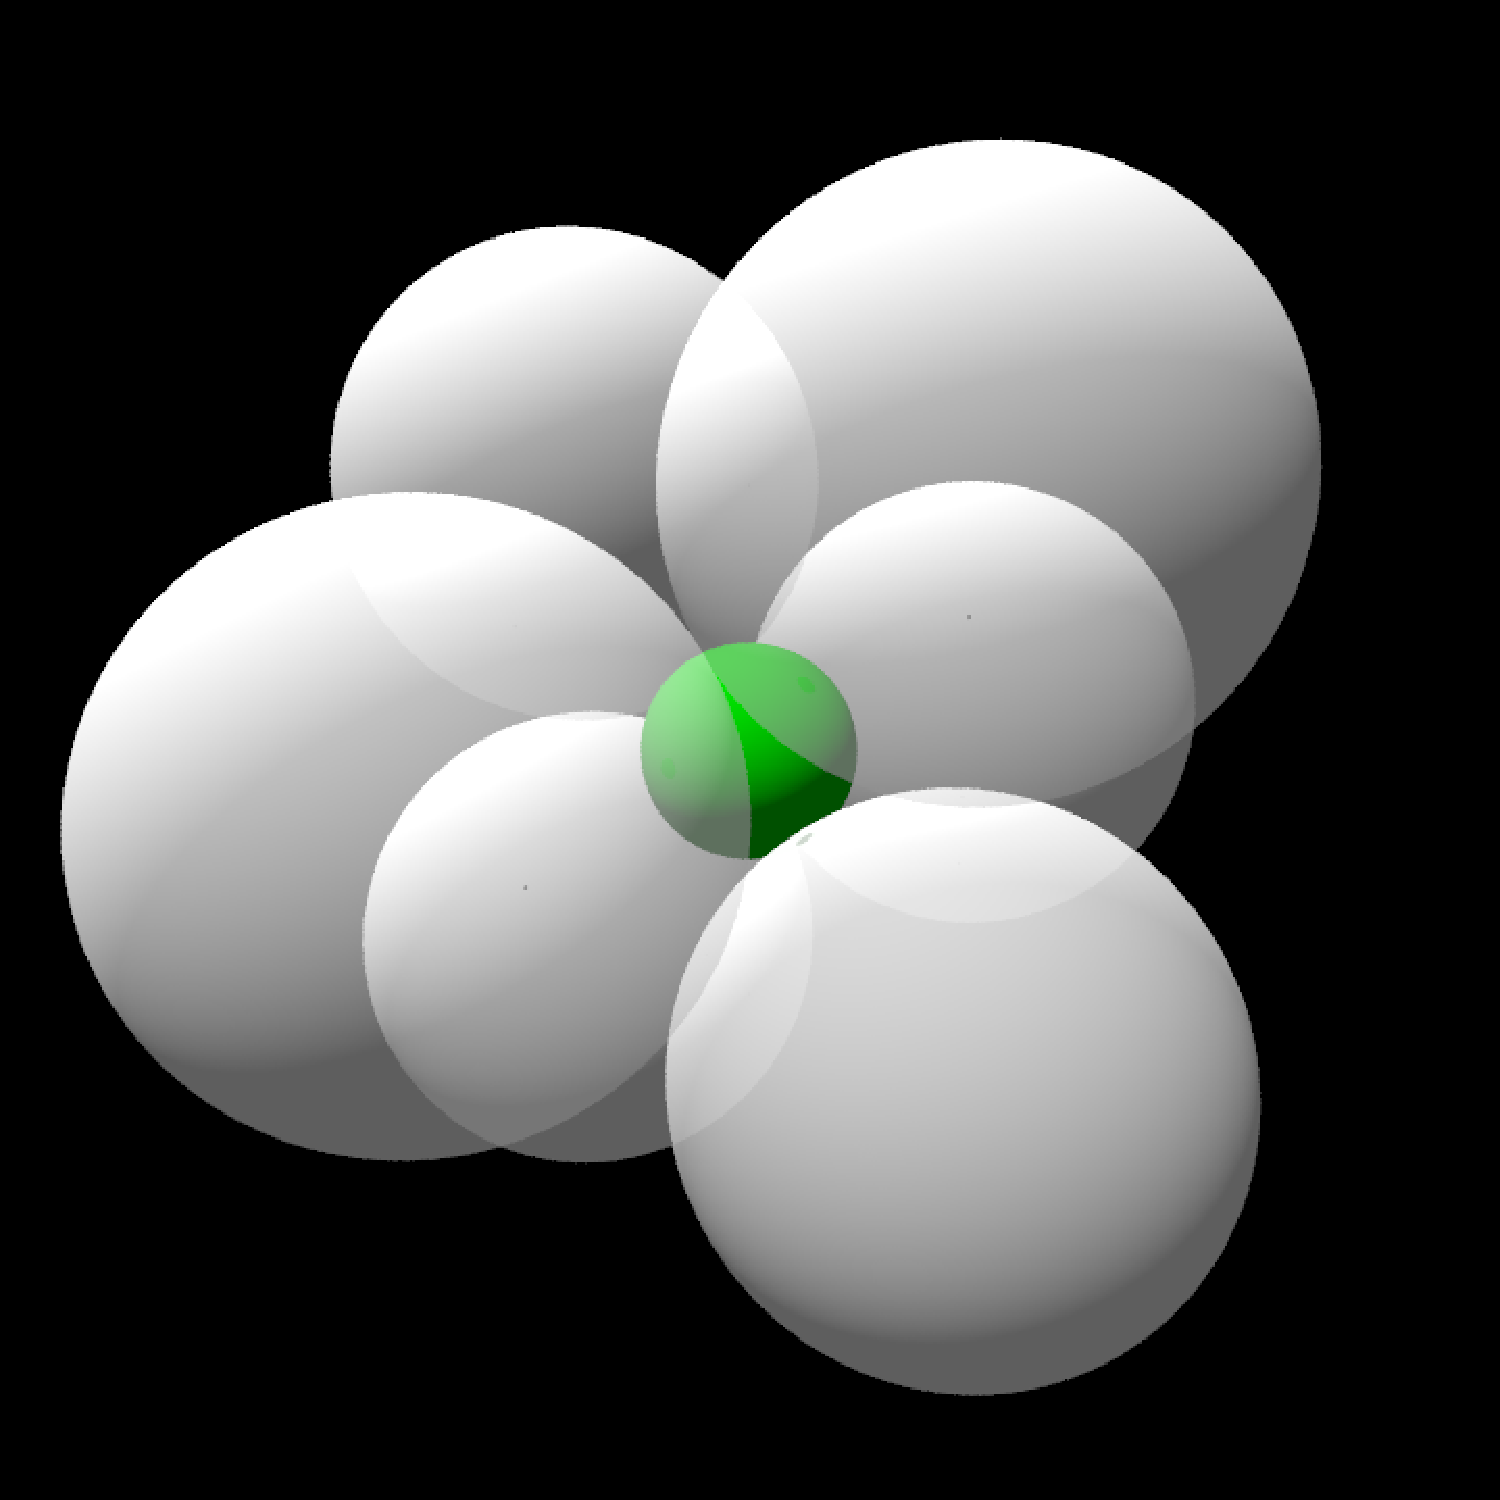
\includegraphics[ height=1.5in, keepaspectratio]{../img/klein/simpleGen.pdf}
   \subcaption{Generator}
   \label{fig:simpleGen3d}
  \end{minipage}
  \begin{minipage}[]{0.49\hsize}
   \center
   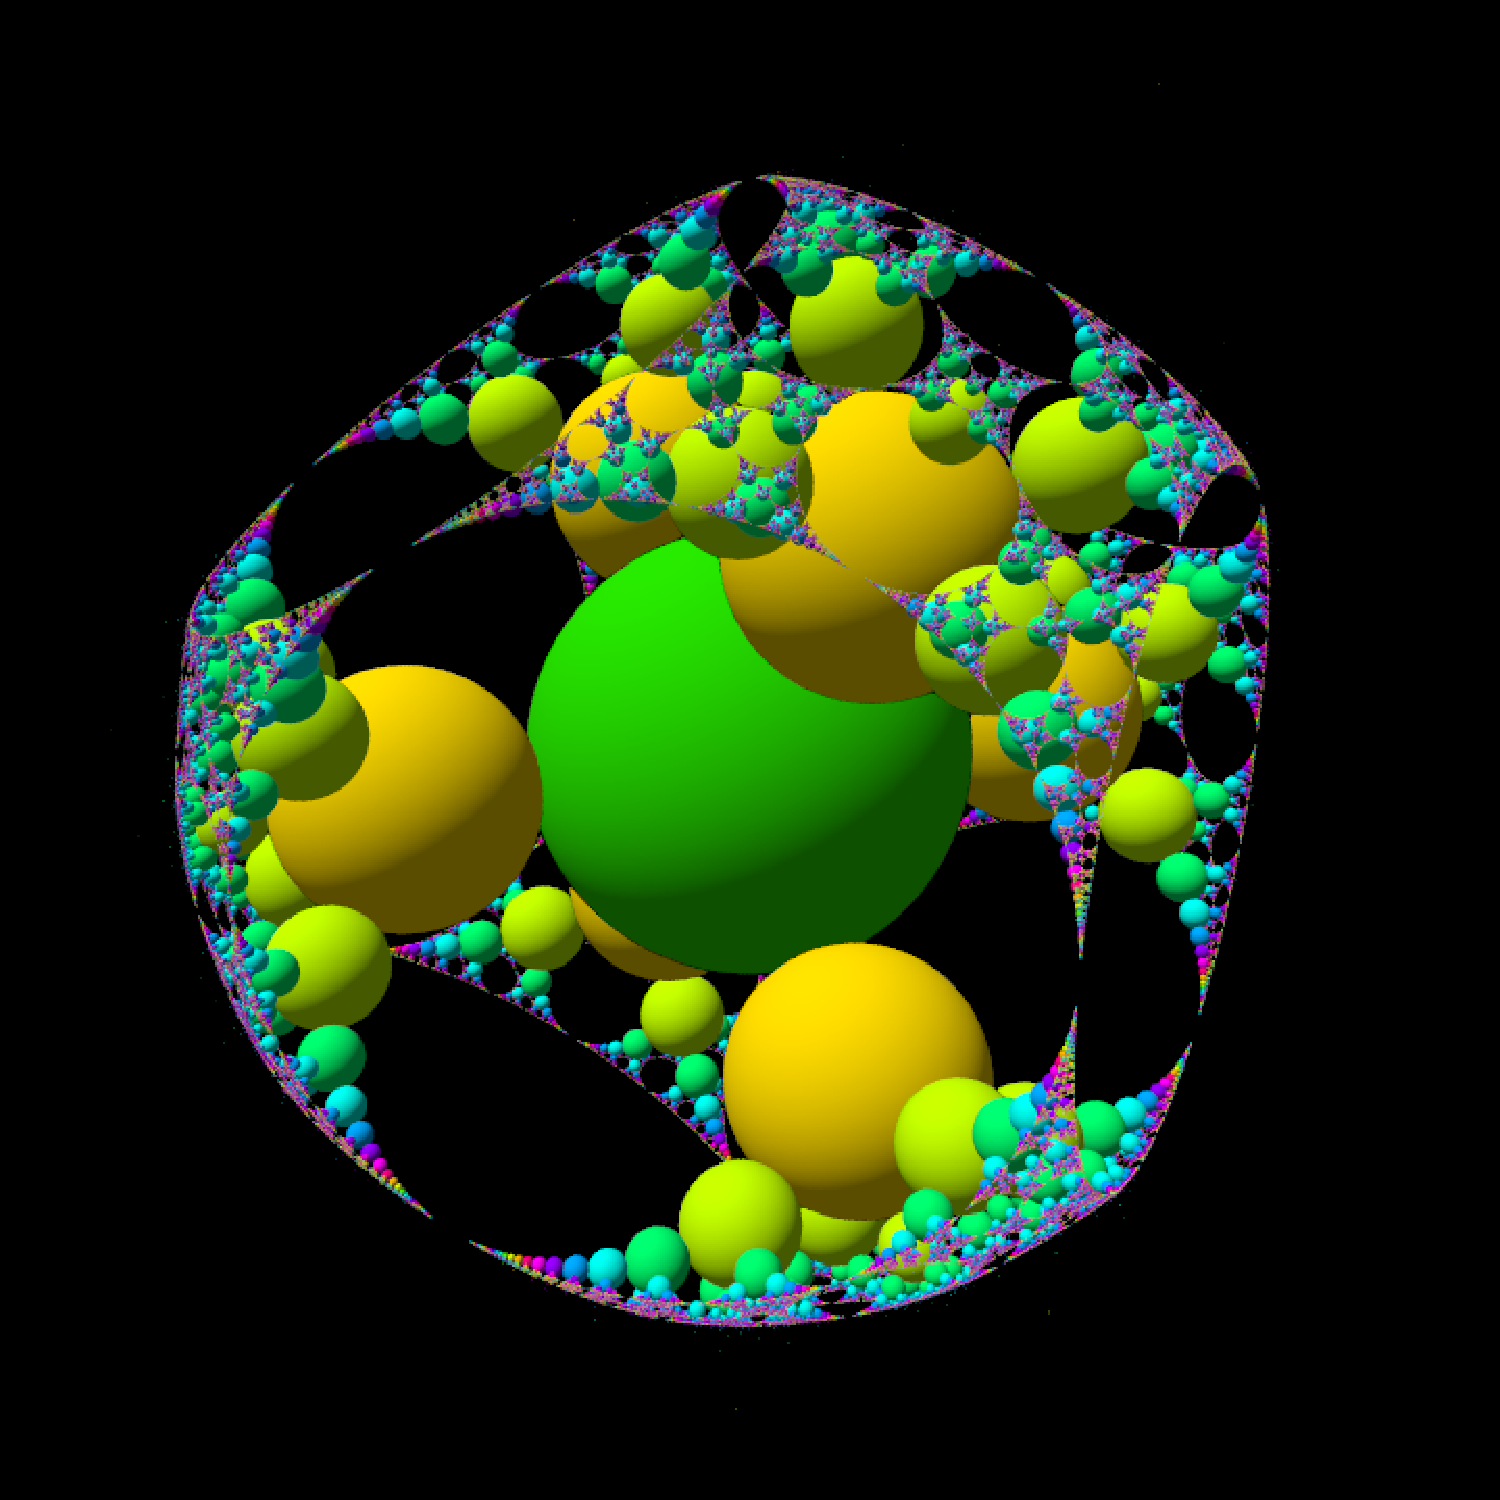
\includegraphics[ height=1.5in, keepaspectratio]{../img/klein/simpleOrbit.pdf}
   \subcaption{Orbit}
   \label{fig:simpleOrb3d}
  \end{minipage}
  \caption{The orbit of the green sphere}
  \label{fig:iis-orb}
 \end{minipage}
 \begin{minipage}[b]{0.5\hsize}
  \center
  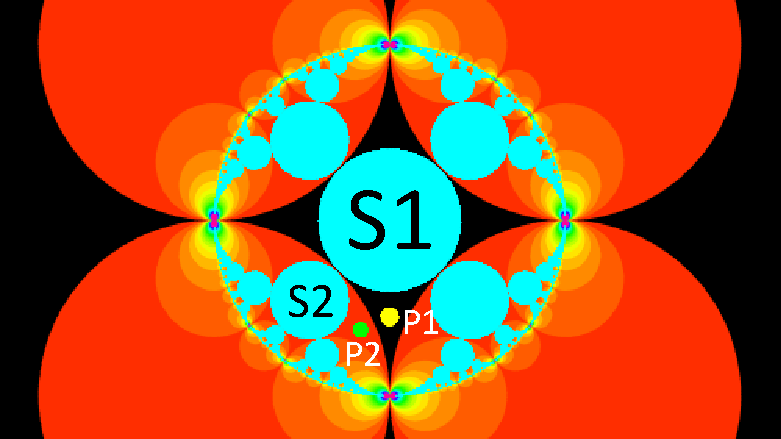
\includegraphics[ height=1.5in, keepaspectratio]{../img/klein/xySlice.pdf}
  \caption{XY-slice image of Figure \ref{fig:iis-orb}}
  \label{fig:xySlice}
 \end{minipage}
\end{figure}

\begin{algorithm}
 \caption{Distance function}
 \label{iis3d}
 \begin{algorithmic}
  \REQUIRE count $= 0$, $d$ = MAX\_DISTANCE, $dr = 1.0$, and coordinates $=$ tipping
  point of the ray
  \FOR{$i=0$ to MAX\_INVERSION}
  \STATE inFundamentalDomain $\leftarrow$ \TRUE
  \FOR{ each Map $G$ in Maps}
  \IF{$G$ is available to coordinates}
  \STATE coordinates $\leftarrow$ $G(\text{coordinates})$
  \STATE $dr \leftarrow dr * $ (Jacobian of $G(\text{coordinates})$)
  \STATE INCREMENT count
  \STATE inFundamentalDomain $\leftarrow$ \FALSE
  \ENDIF
  \ENDFOR
  \IF {isInFundamentalDomain}
  \STATE BREAK for
  \ENDIF
  \ENDFOR
  \FOR{ each BaseSphere $S$ in BaseSpheres}
  \STATE $d \leftarrow$ min($d$, scalingFactor * (distance(coordinates, $S$.center) $-$
  $S$.radius) $/$ (absolute value of $dr$))
  \ENDFOR
  \RETURN $d$
 \end{algorithmic}
\end{algorithm}

\subsection{Geometrical Representation of M\"obius Transformations}

木構造を用いて群を可視化する際には,変換を行列で考えたが,行列表現でメビ
ウス変換を操作することは直観が得にくい.
さらに,四次元クライン群を構成する三次元空間に作用するメビウス変換は, 2×2
四元数行列で表現することができるが,さらにパラメータ数が増大する.
このことは,四次元クライン群の研究があまり進んでいないことの原因にもなっている.
そこで筆者らはすべてのメビウス変換を円や球の反転で構成することを考えた.
円や球を用いることで,生成元と可視化される図形の間の関係性が理解しやすく,
幾何学的な直観を得ることができる.
それに加え,IISを用いることで複雑な生成元をもつ群もリアルタイムに可視化
することができる.
このことは,研究者や学習者だけでなく,フラクタルアーティストにも有益なも
のとなるだろう.
具体的な構成方法などはBridges2017に投稿中である.
また,筆者は円や球の反転で構成される群をインタラクティブに構成するソフト
ウェア, {\it Schottky Link} \footnote{Schottky Link: \url{https://schottky.jp}}を開発している.

\subsection{Other Topics}

この節では, その他のレンダリング手法とクライン群の研究の中でも興味深い図像を見ることができる先行研究を紹介する.

\subsubsection{Other Rendering Methods}
Aaron MontagはIterated Inversion Systemを拡張したHyperbolic Iterated Function Systemによって極限集合を描画することに成功した\cite{hyperbolicIFS}.固定点付近では図に乱れが出るものの,おおむね描画できる.実装はここ\footnote{Kleinian Groups WebGL: \url{https://www-m10.ma.tum.de/bin/view/Lehrstuhl/AaronMontagKleinian}}でみることができる.

また,Jos Ley, Knighty両氏はマスキット群におけるEscape-timeアルゴリズム, Distance Estimationを開発した
\footnote{An escape time algorithm for Kleinian group limit set:\\ \quad
\quad \url{http://www.fractalforums.com/3d-fractal-generation/an-escape-tim-algorithm-for-kleinian-group-limit-sets/}}.
 二次元の極限集合だけでなく,三次元の図像も高速に描画することができる.
荒木・糸\cite{maskit}と同様の設定で, 一方に平行移動を含む2つの放物型変換による群を考えている.
詳細なアルゴリズムに関しては, Jos Ley氏がまとめている\footnote{Mathematical Imagery, An escape-time algorithm for a family of Kleinian groups: \url{http://www.josleys.com/article_show.php?id=221}}.

\subsubsection{Quasi Fuchsian 3-Dimensional Fractals}

Quasi Fuchsian 3-Dimensional Fractalsは阿原・荒木による擬フックス群を三次元に拡張した4次元クライン群である\cite{sphairahedra}\cite{sphairahedraJa}.
前述のフラクタルコミュニティに大きな影響を与えたと言われている.

図\ref{fig:schottky}において, 中央の円盤に囲まれた黒い領域を\emph{円辺形}と呼ぶ.
擬フックス群は円辺形を囲む円盤から生成元を得ることができる.
そこで円辺形を三次元に拡張した\emph{球面体}を用いることで三次元の擬フックス群の形状を求めることができる.
図\ref{fig:sphairahedra}は6つの球に囲まれた球面体のひとつである.
三角柱の面は3つの半径無限大の球に囲まれていると考える.
この球面体をそれを囲む球の反転で移していくことで図\ref{fig:quasiFuchsian}のような形状を得る.

著者によってYouTubeに投稿された動画\footnote{Quasi-fuchsian fractals: \url{https://www.youtube.com/watch?v=3lcO9zRCv-4}}ではこのフラクタルの構成過程をみることができる.
数学的な事項については2016年に蔭山氏がまとめている\cite{kageyama}.
荒木はこのフラクタル図形の物質化についてもまとめている\cite{materializing}.
また,Distance EstimationのアルゴリズムがKnightyにより開発された\footnote{Another 3D Kleinian: \url{http://www.fractalforums.com/ifs-iterated-function-systems/another-3d-kleinian/}}.

\begin{figure}[htbp]
 \begin{minipage}{0.49\hsize}
  \begin{center}
   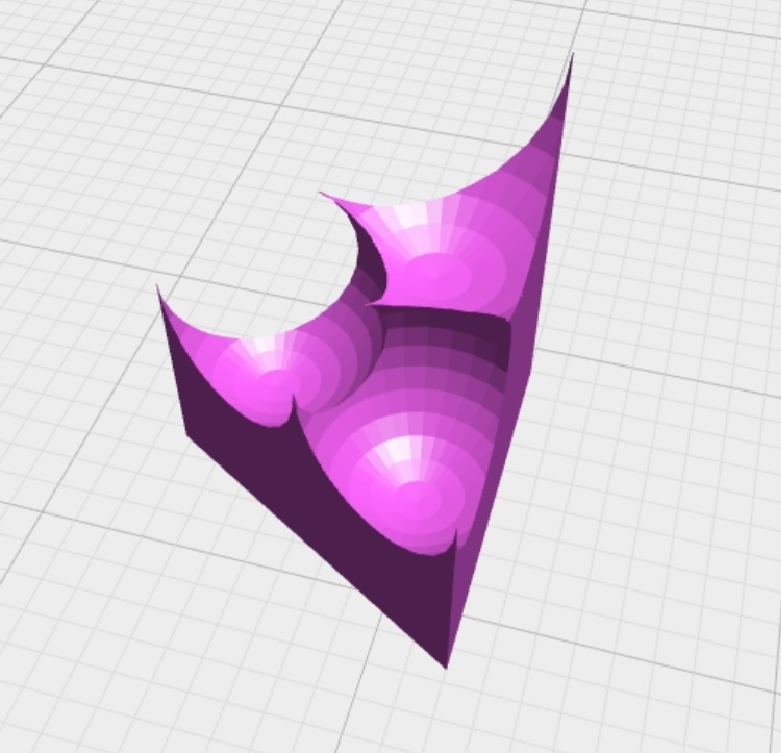
\includegraphics[width=3in, height=3in, keepaspectratio]{../img/klein/sphairahedra.pdf}
   \caption{Sphairahedra}
   \label{fig:sphairahedra}
  \end{center}
 \end{minipage}
 \begin{minipage}{0.49\hsize}
  \begin{center}
   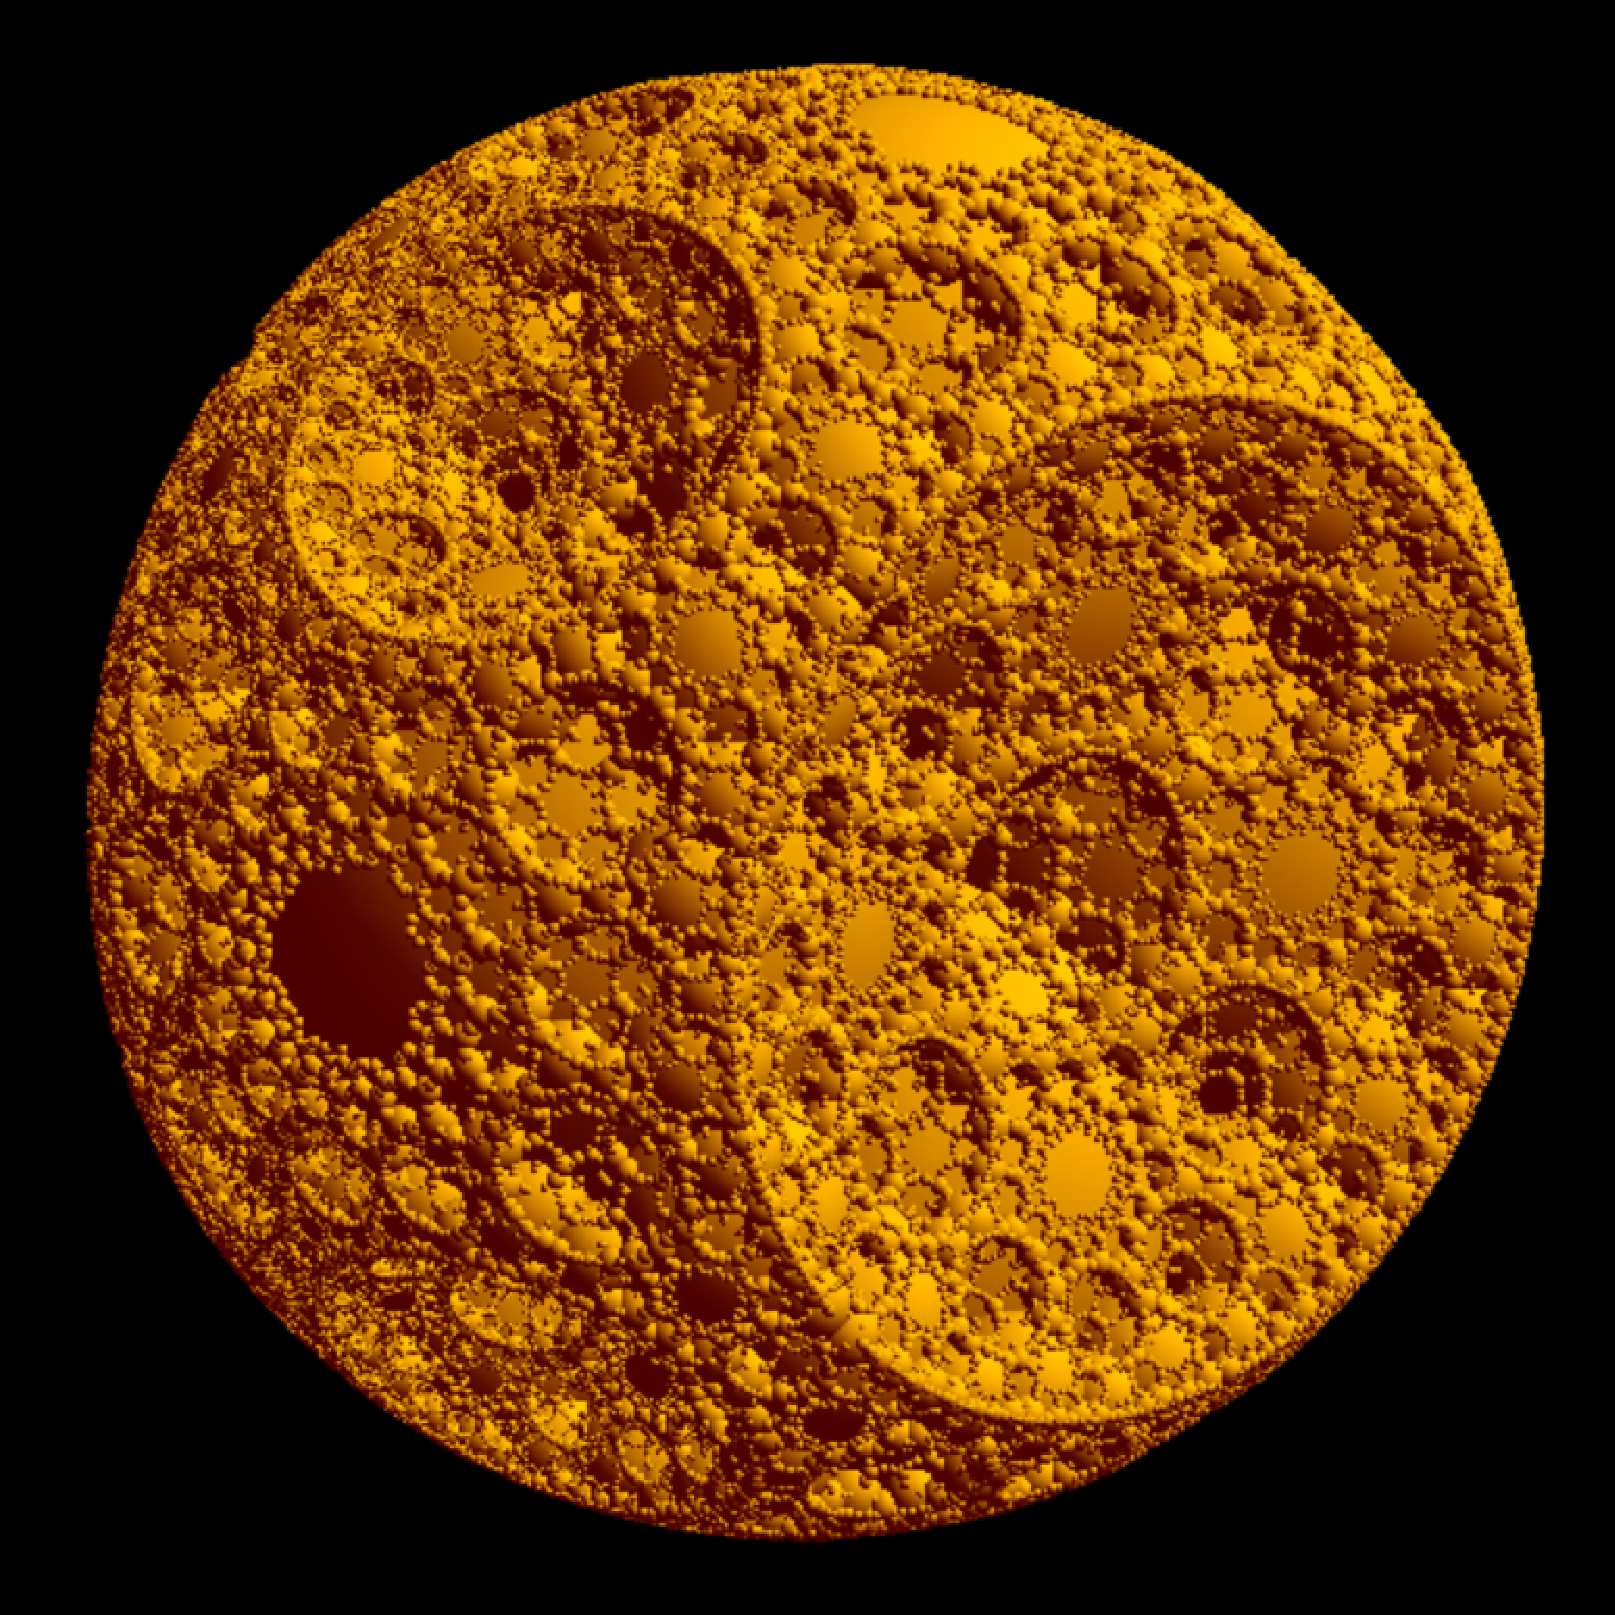
\includegraphics[width=3in, height=3in, keepaspectratio]{../img/klein/quasi-fuchsian.pdf}
   \caption{quasi-fuchsian}
   \label{fig:quasiFuchsian}
  \end{center}
 \end{minipage}
\end{figure}

\subsubsection{Other 4-Dimensional Kleinian Groups}

インドラの真珠で紹介されるクライン群は複素平面にのみ作用するメビウス変換から構成されている.
現在このようなクライン群は, ほぼ研究され尽されてしまった.

しかし, 四元数を用いることで,三次元空間に作用するメビウス変換を定義することができる.
これは$sp^k(1, 1)$と呼ばれ,2x2の四元数行列で表現される.
四元数で構成されるメビウス変換とその分類は佐久川による\cite{sakugawaMaster}や\cite{accidentalParabolic}にまとまっている.佐久川氏は,三次元空間上で捩じりが加わるようなメビウス変換を\emph{複合放物型}({\it Compund Parabolic}), \emph{複合斜航型}({\it Compound Loxodromic})と分類した.
図\ref{fig:sakugawa}は佐久川氏による複合放物型変換を含む群のレシピによる群の極限集合を描画したものである.
放物型変換である平行移動に回転が加わることで複合放物型変換となる.

荒木・糸両氏はマスキット群を四次元クライン群に拡張した\cite{maskit}.幾何学的性質をうまく使うことで,四元数の計算を避けている.レンダリングされた極限集合は糸氏のWebページ\footnote{4-dimensional Kleinian punctured torus groups: \url{http://www.math.nagoya-u.ac.jp/~itoken/3d-maskit/3d-maskit.html}}や論文中で見ることができる.佐久川氏はこの群の四元数表示を導出した\cite{sakugawa4d}.

三浦氏は3つ以上の生成元による4次元クライン群をモジュラー群から構成することを試みた\cite{miura}.筆者はこの論文における数値実験と可視化を行った.

\begin{figure}[h!tbp]
 \begin{subfigure}{0.49\hsize}
   \begin{center}
    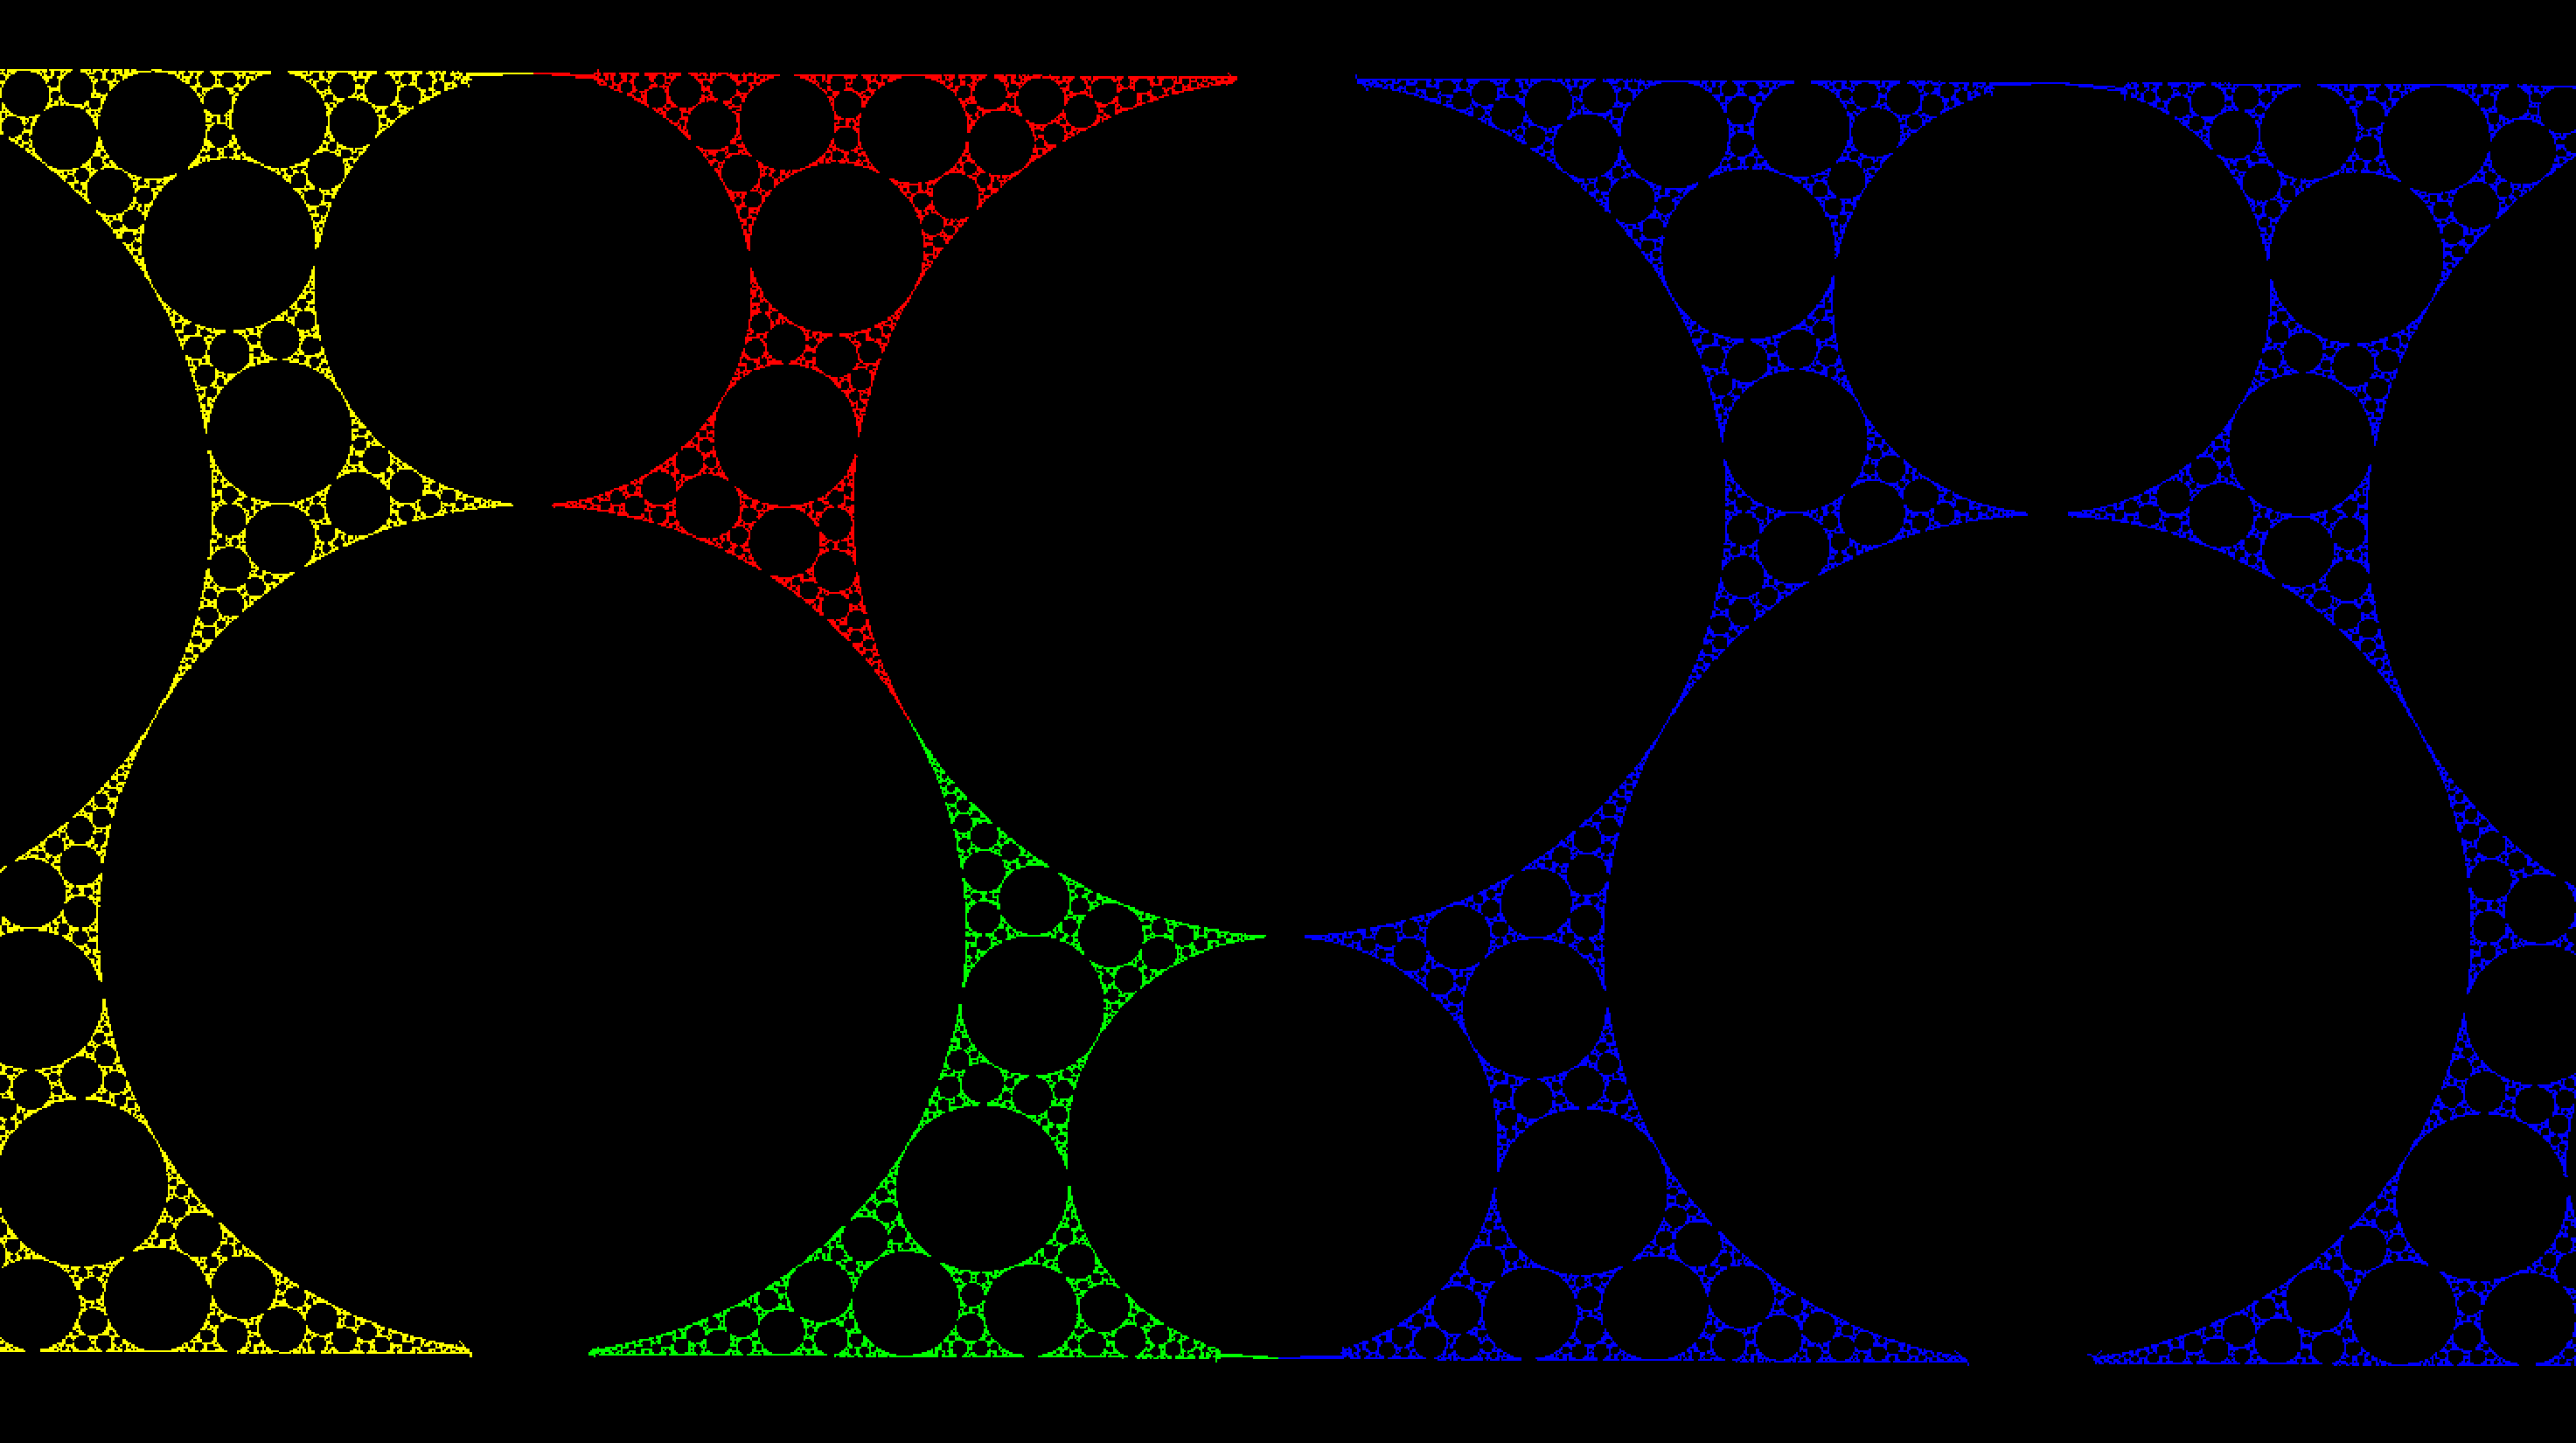
\includegraphics[width=3in, height=3in, keepaspectratio]{../img/klein/sakugawa1.pdf}
    \caption{}
    \label{fig:sakugawa1}
   \end{center}
 \end{subfigure}
 \hspace*{\fill}
 \begin{subfigure}{0.49\hsize}
   \begin{center}
    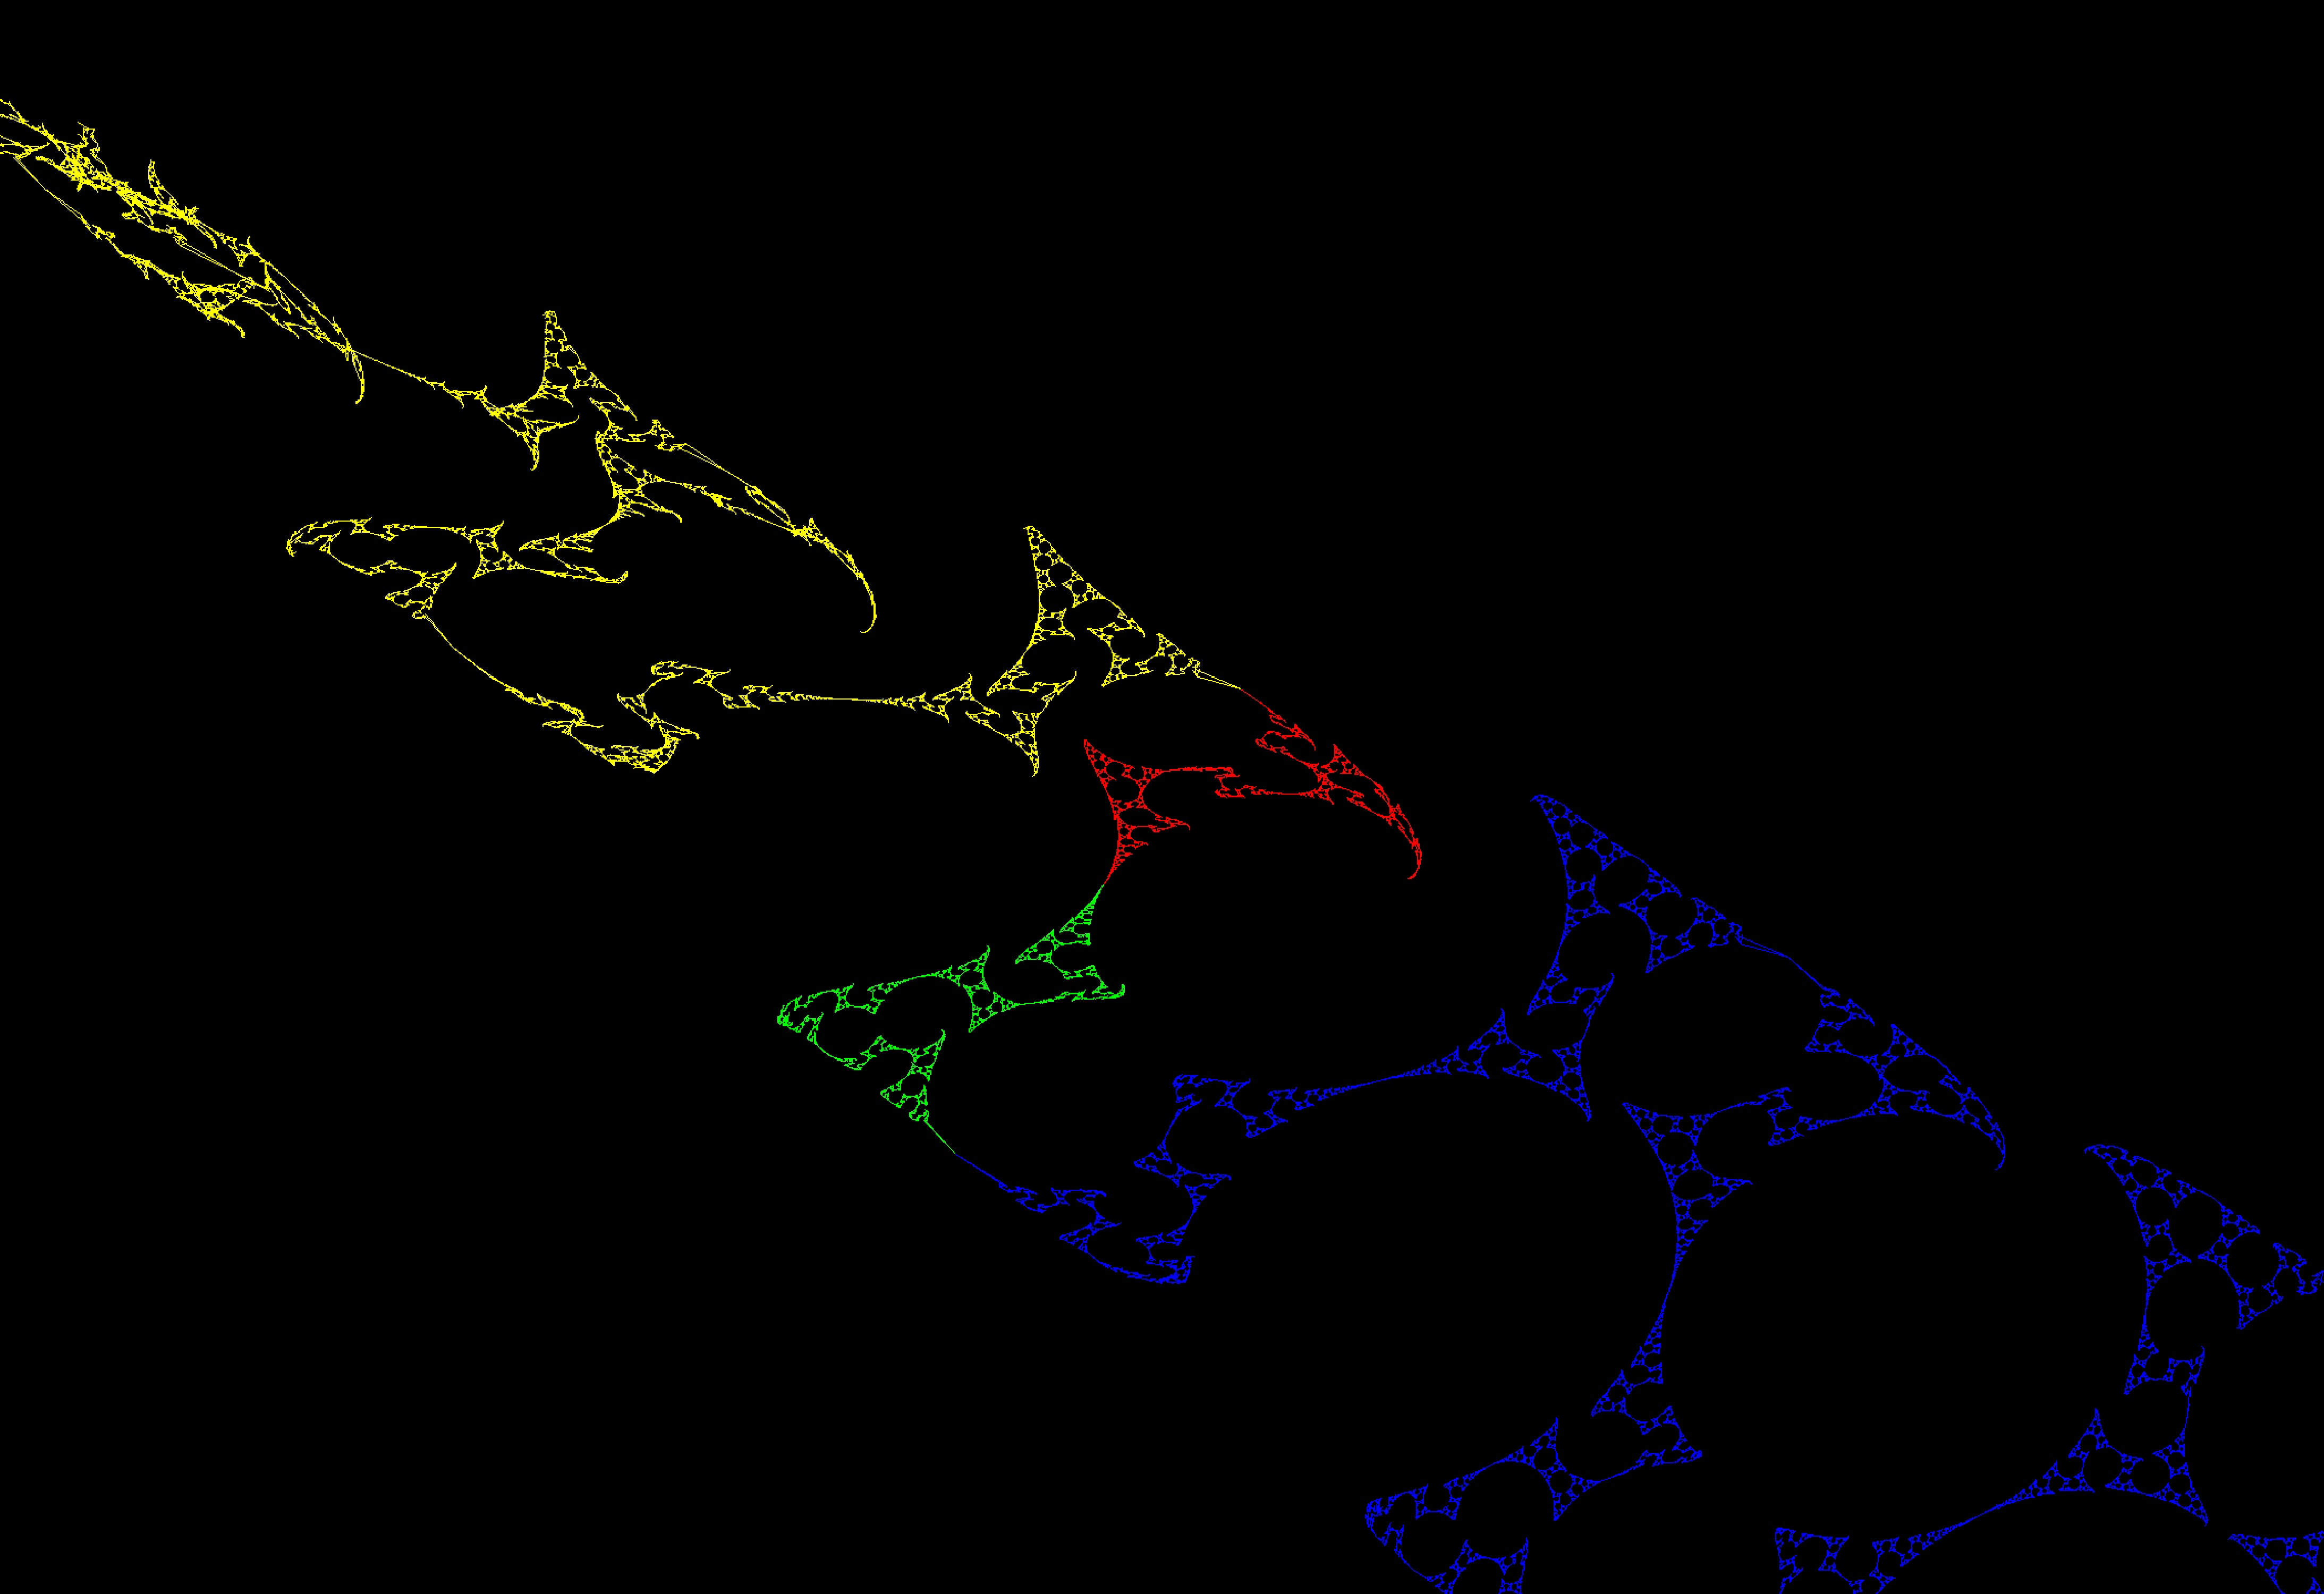
\includegraphics[width=3in, height=3in, keepaspectratio]{../img/klein/sakugawa2.pdf}
    \caption{}
    \label{fig:sakugawa2}
   \end{center}
 \end{subfigure}
 \caption{The limit set of the 4-Dimensional Kleinian Groups}
 \label{fig:sakugawa}
\end{figure}

\subsubsection{Once Punctured Torus Groups}
{\it Once Punctured Torus Groups}はクライン群の一種である.{\it OPTi}\footnote{OPTi: \url{http://delta-mat.ist.osaka-u.ac.jp/OPTi/index.html}}という描画ソフトウェアが有名である.
描画\cite{OPTiDrawing}や離散性判定\cite{OPTiDiscrete}のためのアルゴリズムが和田によりまとめられている.
このスライス領域はベアズスライスとよばれる.
Once Punctured Torus Groupsの研究はOPTiによって進歩した.
図\ref{fig:opt}のように, 平行移動の生成元をもつため, 極限集合は比較的高速に描画することができる.

\begin{figure}[htbp]
 \begin{center}
      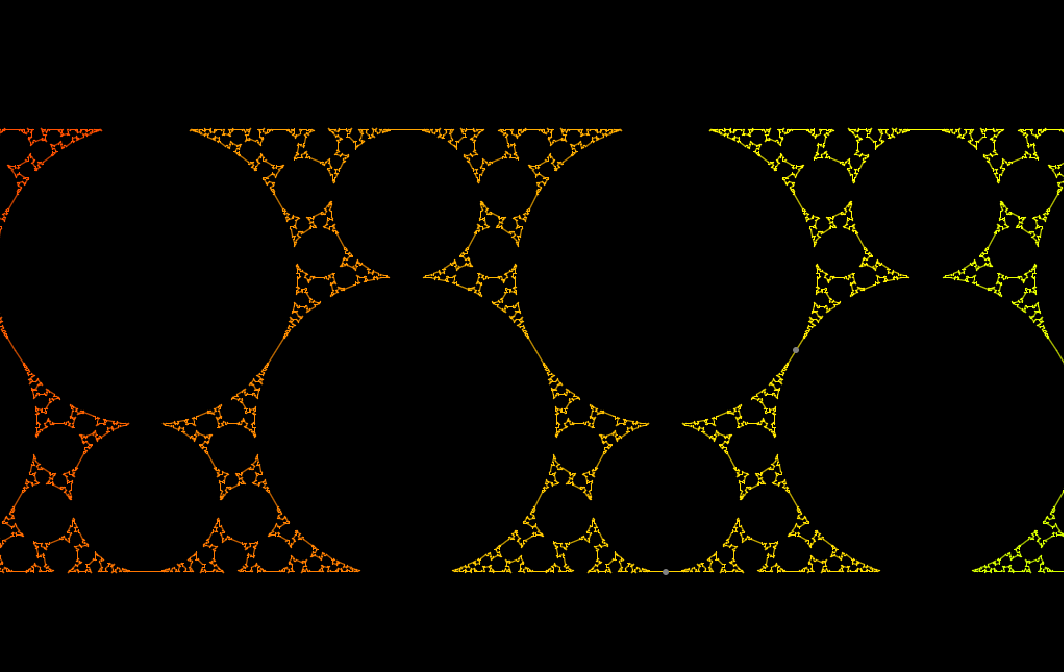
\includegraphics[width=3in, height=3in, keepaspectratio]{../img/klein/optg.pdf}
    \caption{The Limit Set of the once punctured torus groups}
    \label{fig:opt}
 \end{center}
\end{figure}

\subsection{Further Readings}
この章の最後に,クライン群のより数学的な背景を学習するための書籍をいくつか挙げておく.
『双曲幾何学への招待』\cite{invitation}は絶版であるが双曲幾何学の基本事項がまとまっている.
クライン群のより数学的内容に踏み込んだ書籍には『双曲多様体とクライン群』\cite{manifold}や『Outer Circles』\cite{outerCircles}がある.
また, レクチャーノート集に『Kleinian Group and Hyperbolic 3-Manifolds』\cite{kleinianGroupsAndHyperbolic3-Manifolds}や
『Spaces of Kleinian Groups』\cite{space}がある.